\chapter{Auswertung zum \tit{Corpus der altdeutschen Originalurkunden}}
\label{ch:caoanalyse}

Im Folgenden werden zunächst die aus dem \citetitle*{cao} (\CAO{})
exzerpierten Belege zu \norm{bėide} näher untersucht. Zunächst erfolgt eine
kurze geografische Einordnung der Belege, um sicherzustellen, dass der Großteil
davon in das schreib\-dialektal relevante Gebiet entfällt. Durch die Kartierung
wird außerdem deutlich, welche Regionen gegebenenfalls über- oder
unter\-repräsentiert sind. Danach erfolgt die Untersuchung in Hinsicht auf das
Auftreten der Wortformen \norm{bėide} und \norm{bėidiu} als determinierender
Quantor in Abhängigkeit von Personenmerkmalen in unterschiedlichen
syntaktischen Kontexten. Daran schließt sich eine Untersuchung nach Distanz
zwischen Controller und Target an. Am Schluss des Kapitels steht der Vergleich
zwischen \norm{bėide} als Konjunk\-tion in der Konstruktion
\norm{bėide \dots\ unde} `sowohl \dots\ als auch'.

\section{Geografische Verteilung der gesammelten Belege}

Die Karte in \cref{fig:beidemapcao} zeigt die Abdeckung des gesammelten
Belegmaterials in Bezug auf die Anzahl der Belege für \norm{bėide} pro
Ausstellungsort für Quantor und Konjunktion; die Liste der ausgewerteten
Urkunden befindet sich in \cref{subsec:ausgewurk}. Der alemannische Raum ist
breit abgedeckt. Besonders Straßburg (22~Belege), Zürich (15), Basel (15) und
Freiburg i.\,Br.\ (12) stechen dabei heraus. Im Schwäbischen dominiert Augsburg
(29); im Bairischen tut sich vor allem das Mittelbairische mit den großen
Städten Wien (23) und Salzburg (14) hervor. Ebenfalls dem Belegmaterial
geschuldet ist die Tatsache, dass die Belegdichte nördlich des Mains gegen Null
tendiert, abgesehen von Köln (25). Da davon auszugehen ist, dass das
untersuchte Phänomen ohnehin nur das Oberdeutsche betrifft
\autocite[181--184]{ksw2}, stellt die Verteilung der Belege kein größeres
Problem für die Auswertung dar.

\begin{figure}
\centering
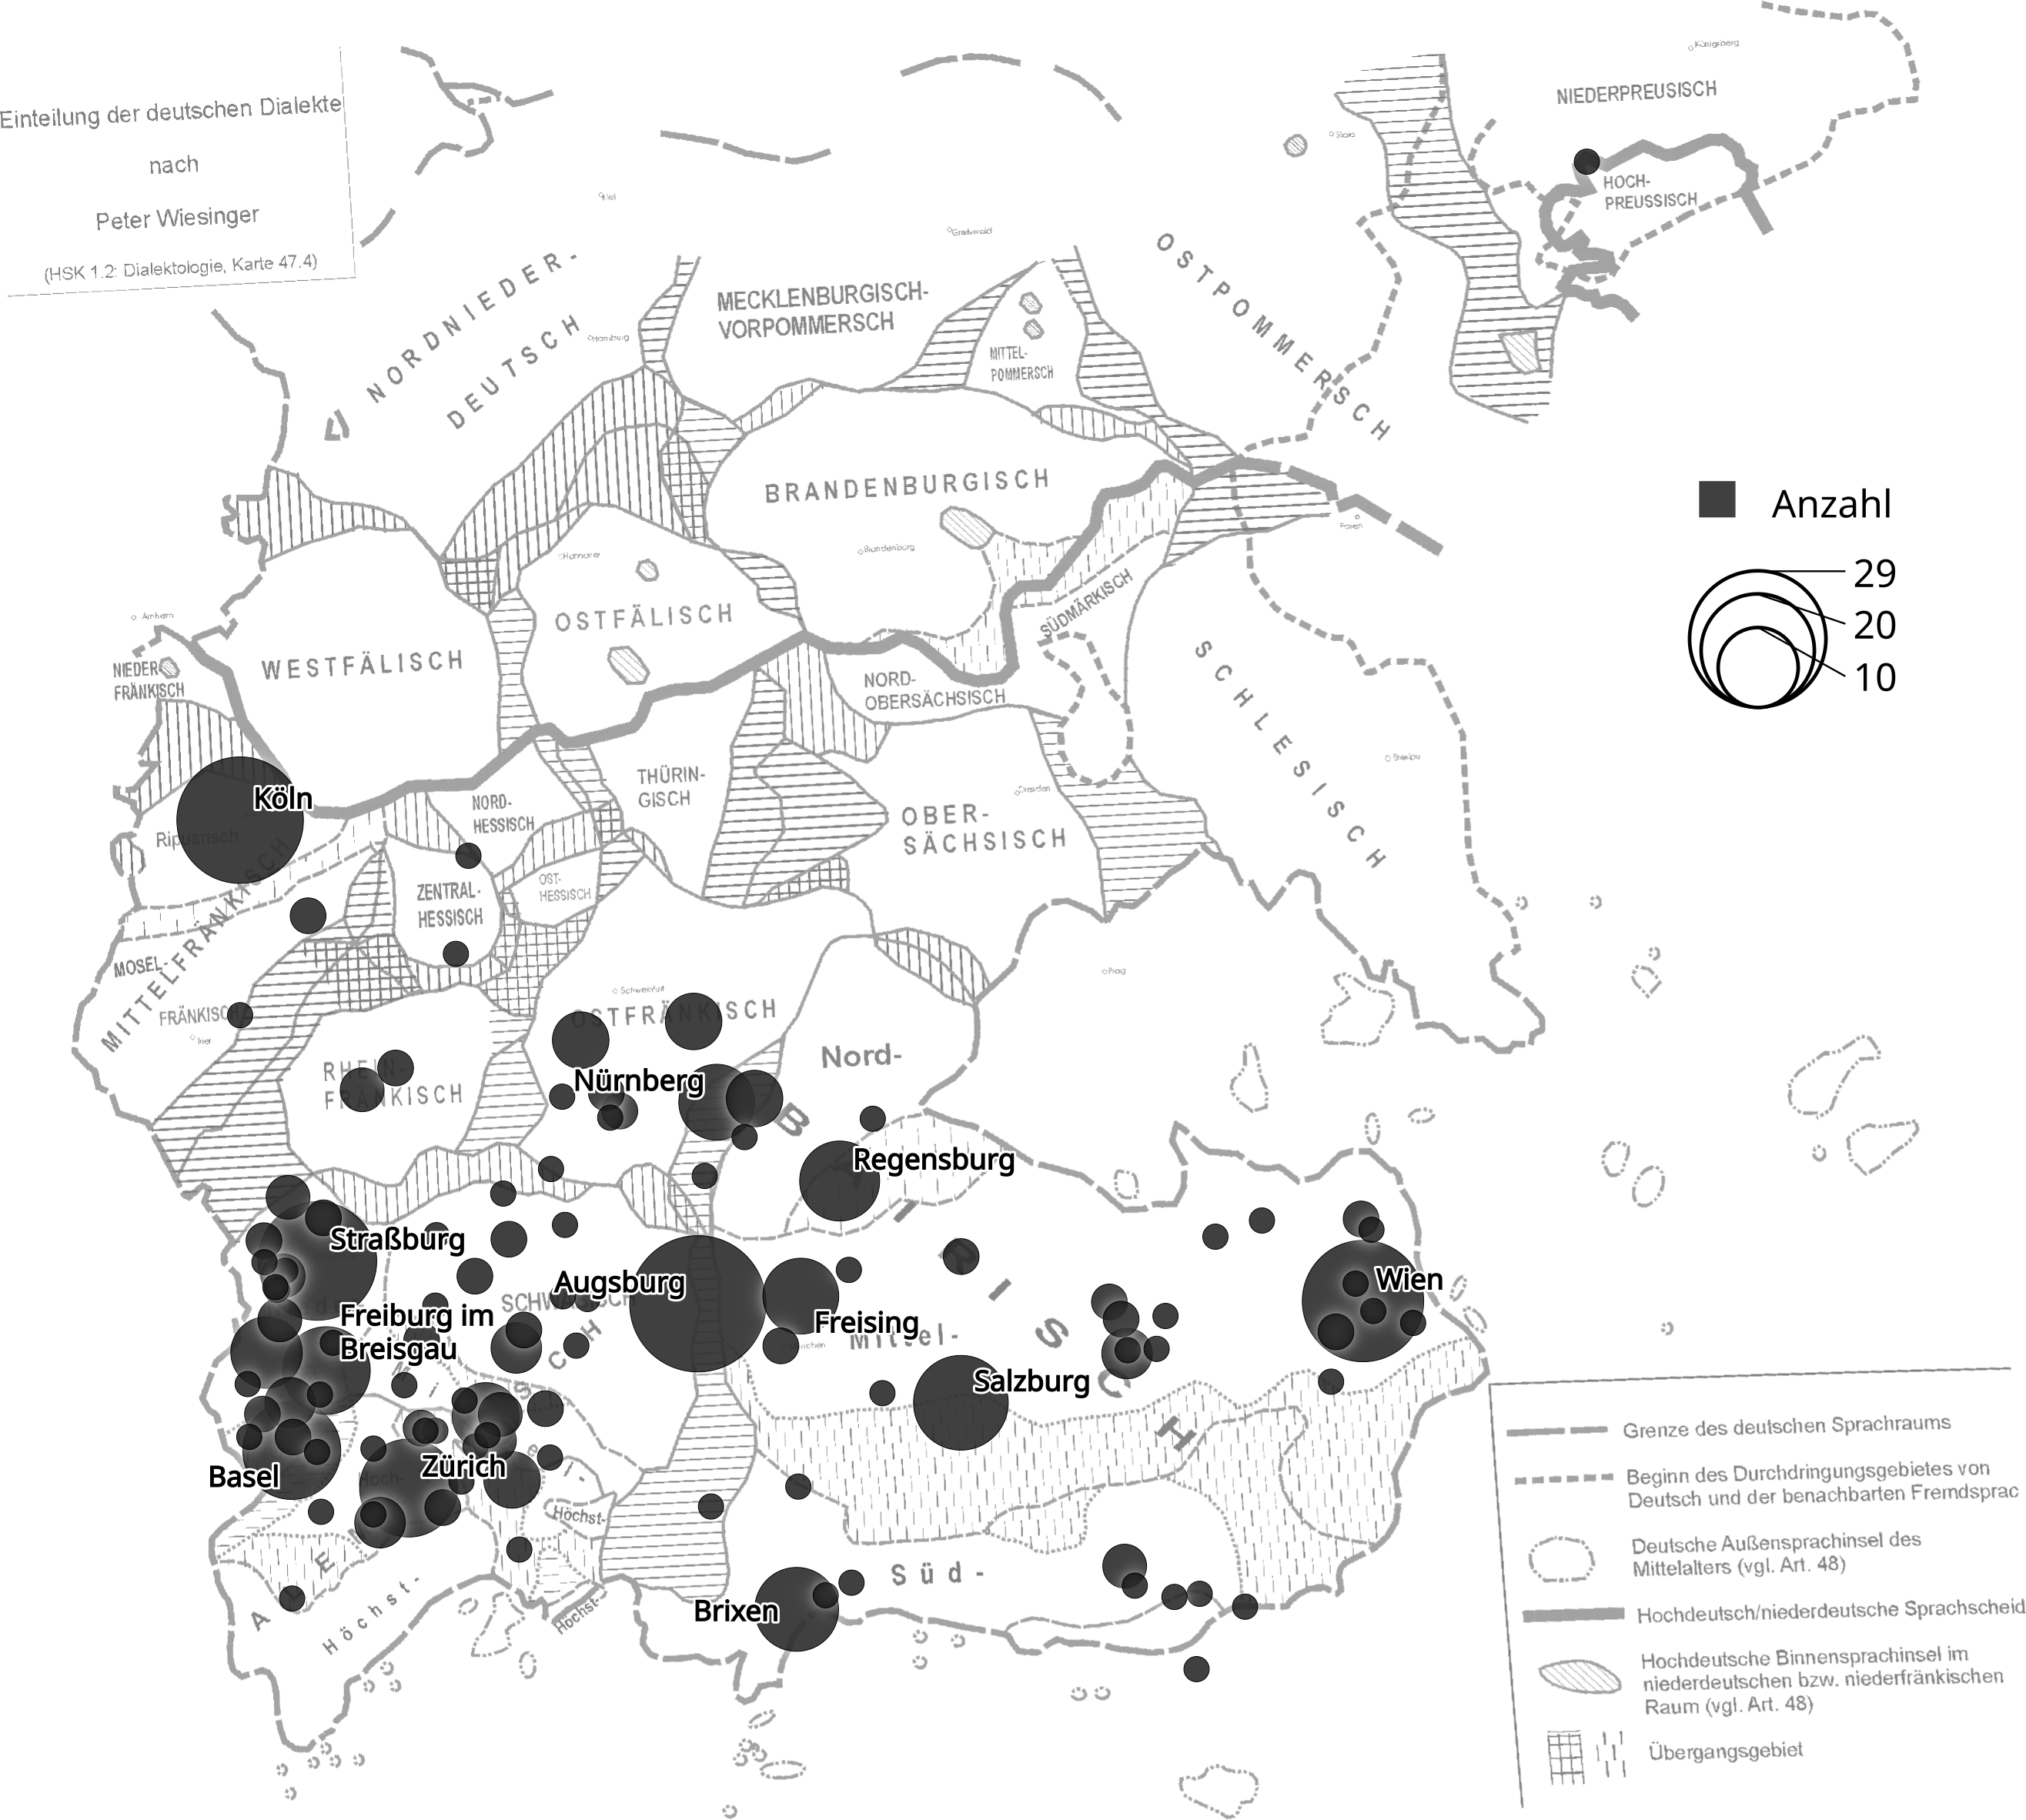
\includegraphics[
	width=\linewidth,
	height=.75\textheight,
	keepaspectratio
]{./figures/2021-05-11_cao_beide_iu-per-place-quant+conj.png}
\caption{Anzahl der Belege für mhd.\ \norm{bėide} pro Ausstellungs\-ort
im \CAO{}\nocite{wiesinger1983:rede}}
\label{fig:beidemapcao}
\end{figure}

Die 35 westmitteldeutschen Belege aus Köln (25~Belege), Burg Altleiningen
(Kr.~Bad Dürkheim; 3), Sayn (Kr.~Mayen-Koblenz; 2), Worms (2), Rüdigheim
(Kr.~Marburg-Biedenkopf; 1), Schloss Naumburg (Main-Kinzig-Kreis; 1) und
Veldenz (Kr.~Bernkastel-Wittlich; 1) zeigen den Angaben der Grammatik gemäß
keine Variation zwischen \norm{bėide}- und \norm{bėidiu}-Formen. Diese Belege
werden im weiteren Verlauf von der Analyse ausgeschlossen; die betroffenen
Urkunden werden in \cref{subsec:ausgesurk} aufgeführt. Bei der Besprechung
individueller Belege finden sich im Alemannischen noch weitere Fälle, in denen
am Ort nach kursorischer Durchsicht der Belege für \norm{e}- und
\norm{iu}-Formen in Urkundentexten des jeweiligen Ortes im \CAO{}
keine Variation vorliegt (vgl. auch \cref{sec:adjdeclcao} zu Straßburg). Da
nachfolgend aufgrund der Anzahl der Belege nicht sämtliche von ihnen einzeln
besprochen werden können, ist mit weiteren solchen Fällen gewissermaßen als
\q*{Grundrauschen} zu rechnen.

\needspace{3\baselineskip}
\section{Targets nach Personenmerkmalen des Controllers}
\label{sec:caotargpers}

\subsection{Nominale Controller}
\subsubsection{Kombinierte nominale Controller}
\label{subsubsec:perscombsgnp}

Zunächst werden \norm{bėide} und \norm{bėidiu} in direkter Abhängigkeit von
koordinierten nominalen Ausdrücken (Substantive, Pronomen) wie zum Beispiel
\norm{her Rvͦdiger vnd ſin hovſfrowe} `Herr Rüdiger und seine Ehefrau' in
\cref{ex:beid2coordncao1} näher betrachtet. Dabei werden Kombinationen von
Personalpronomen und Eigenname wie \norm{ich unde Ulrich} an dieser Stelle
mitgezählt, da auch diese eine nominale Kategorie darstellen, insofern sie
sich im Kontext dieser Untersuchung regelmäßig auf ein substantivisches
Antezedens beziehen und dessen Personenmerkmale reflektieren.
% %
% 	\footnote{Formal ist die Kategorie \xhead{D}, die im Deutschen die Pronomen
% 	enthält, das funktionale Äquivalent zur lexikalischen Kategorie \xhead{N}
% 	der Substantive \autocite[vgl.~z.\,B.][135--138]{bresnanetal2016}.}
% %
Zwei Belege werden in \cref{ex:beid2coordncao1} angeführt. Das beigefügte
Schema verdeutlicht den syntaktischen Kontext.

\begin{exe}
\ex \label{ex:beid2coordncao1}
\begin{xlist}
	\ex \label{ex:beid2coordncao1_1}
		\begin{tikzpicture}[baseline=(1a_lb.base)]
			\node at (0,2)  (1a)    {\norm{her Rvͦdiger}};
			\node           (1a_box)[draw,rectangle,fit=(1a)] {};
			\node           (1a_lb) [above=.5ex of 1a_box, font=\mynodefont]
		                            {Controller 1};

			\node at (0,0)  (1b)    {\norm{ſin hovſfrowe}};
			\node           (1b_box)[draw,rectangle,fit=(1b)] {};
			\node           (1b_lb) [above=.5ex of 1b_box, font=\mynodefont]
		                            {Controller 2};

			\node at (3,1) (2)      {\norm{bediv}};
			\draw (2) node (2_box)  [draw,rectangle,fit=(2)] {};
			\node (2_lb)   [above=.5ex of 2_box, font=\mynodefont] {Target};

			\draw [-latex] (1a_box) to [out=east, in=west] (2_box);
			\draw [-latex] (1b_box) to [out=east, in=west] (2_box);
		\end{tikzpicture}

	\sn \gll swenne aber her Rvͦdiger vnd ſin
			hovſfrowe bediv niht enſint\\
			so=wenn aber Herr Rüdiger[\Nom.\Sg.\MascM] und sein
			Ehefrau[\Nom.\Sg.\FemF] beide-\Nom.\Pl.\NeutMF.\St{} nicht
			\Neg=sind\\
			\trans `Wenn aber irgendwann Herr Rüdiger und seine Ehefrau
				beide nicht \textins{mehr} sind'
				\parencites(Nr.~3262, Regensburg, 1299)[425,13--14]{cao4}

	\ex \label{ex:beid2coordncao1_2}
		\gll Diſ dingeſ gezuga ſint · Ruͦd · von der palma
			min Oͤhen · vͦlrich von Grvͤnenberch min Oͤhen
			bedu Jungherren \\
			% · hug von waltherſwile · \textelp{} \\
			Dies Verhandlung-\Gen.\Sg.\NeutI{} Zeugen sind {}
			\lit{Ruͦd}[\Nom.\Sg.\MascM] {} von der Palme mein Oheim {}
			Ulrich[\Nom.\Sg.\MascM] von Grünenberg mein Oheim
			beide-\Nom.\Pl.\NeutM.\St{} Jungherren[\Nom.\Pl.\MascM] \\
			% {} Hug von Walterswil {} {} \\
		\trans `Zeugen dieser Verhandlung sind: \lit{Ruͦd} von der Palme,
			mein Onkel, Ulrich von Grünenberg, mein Onkel -- beide Junker --
			% Hug von Walterswil, 
			\textelp{}'
				\parencites(Nr.~2915, Kl.~St.~Urban, Kt.~Luzern, 1298)[213,33--35]{cao4}
\end{xlist}
\end{exe}

Daneben liegen noch die drei Belege in \cref{ex:beid2coordncao2} vor, die aus
der regulären Auswertung ausgeschlossen wurden, da bei ihnen die Flexion des
Targets vor einem Wort steht, das mit einem Vokal beginnt, also in einer
Hiatusposition steht \autocites[vgl.][90--91]{askedal1973}[191--193,
201]{gjelsten1980}. Dies hat bei den Prosatexten des \CAO{} jedoch
keine große Auswirkung (vgl.~\cref{phsec:caohiatus}), sodass diese Belege
aufgrund der geringen Anzahl zur Analyse hinzugezogen werden können, zumal sie
ansonsten einschlägig sind. In \cref{tab:combnomctrl} erscheinen sie grau
gedruckt.

\begin{exe}
\ex \label{ex:beid2coordncao2}
	\begin{xlist}
	\ex \label{ex:beid2coordncao2_1}
		\gll wir · krafte von hohenloch · vn̄ · wir ludewic
			von durne · geloben baide vf vnſern eit \\
			\Fsg\subM.\Hon.\Nom{} {} Kraft von Hohenlohe {} und {}
			\Fsg\subM.\Hon.\Nom{} Ludwig von Durne {} geloben
			beide-\Nom.\Pl.\MascM.\St{} auf unseren Eid \\
		\trans `Wir, Kraft von Hohenlohe, und Wir, Ludwig von Durne,
			geloben beide Kraft unseres Eides'
			\parencites(Nr.~2529, Burg Hohlach, Kr.~Neustadt an der Aisch-Bad Windsheim)[563,5--6]{cao3}

	\ex \label{ex:beid2coordncao2_2}
		\gll Jch seibot von freihaim / vnd fraͮwe Peters mein
			Havſfraͮwe / veriehen beidev vnd tuͦn chvnt \\
			\Fsg\subM.\Nom{} Seibot von Freiheim {} und Frau
			Peters[\Nom.\Sg.\FemF] mein Ehefrau {} bekennen
			beide-\Nom.\Pl.\NeutMF.\St{} und tun kund \\
		\trans `Ich, Seibot von Freiheim, und Frau Peters, meine Ehefrau,
			bekennen beide und machen bekannt'
			\parencites(Nr.~3248, München, 1299)[416,23]{cao4}

	\ex \label{ex:beid2coordncao2_3}
		\gll minen hof \textelp{} verkaufft han mit dem
			zehenden \textelp{}, beidev vnuerſchaidenlichen
			fvͤr reht aigen \\
			meinen Hof[\Acc.\Sg.\MascI] {} verkauft habe mit dem
			Zehnt-\Dat.\Sg.\MascI{} {} beide-\Acc.\Pl.\NeutI.\St{}
			gleichermaßen für rechtmäßig Eigentum \\
		\trans `meinen Hof verkauft habe mit dem Zehnten \textelp{}, beide
			gleichermaßen zum rechtmäßigen Eigentum'
			\parencites(Nr.~N~241, Augsburg, 1283)[195,37--39]{cao5}
	\end{xlist}
\end{exe}

\cref{tab:combnomctrl} fasst die Personenmerkmale der in
\cref{ex:beid2coordncao1,ex:beid2coordncao2} zitierten Beispiele zusammen und
gibt die Häufigkeiten der jeweiligen Kongruenzformen des Quantors pro
Merkmalskombination an. Zur Angabe der belegten Flexionstypen ist anzumerken,
dass die Spalte \norm{bėidiu} gemäß den Ergebnissen in \cref{sec:adjdeclcao}
zur regionalen Ausprägung von \norm{-e} und \norm{-iu} in der starken
Adjektivdeklination im \CAO{} die verschiedenen als äquivalent
angesehenen Grafien der Flexionsendung zusammenfasst. Dies sind:
\lit{iu/iv},
\lit{îv},
\lit{ivͤ},
\lit{iͤv},
\lit{uͥ/vͥ},
\lit{ú/v́},
\lit{v̓},
\lit{u/v},
\lit{eiw},
\lit{eu/ev}
sowie
\lit{i}.

\begin{table}
\centering
\caption{Flexion nach Personenmerkmalen der kombinierten nominalen Controller}
\begin{tabular}{l l r r}
\toprule
Controller 1
	& Controller 2
	& bėide
	& bėidiu
	\\
\midrule
\Tsg.\MascM      & \Tsg.\MascM       &        & 1        \\
\Tsg.\MascM      & \Tsg.\FemF        &        & 1        \\
\midrule
\mc{2}{l}{Summe}                     &        & 2        \\
\midrule
\midrule
\gr{\Fsg\subM}   & \gr{\Fsg\subM}    & \gr{1} &          \\
\gr{\Fsg\subM}   & \gr{\Tsg.\FemF}   &        & \gr{1}   \\
\gr{\Tsg.\MascI} & \gr{\Tsg.\MascI}  &        & \gr{1}   \\
\midrule
\mc{2}{l}{\gr{Summe}}                & \gr{1} & \gr{2}   \\
\bottomrule
\end{tabular}
\label{tab:combnomctrl}
\end{table}

Die niedrige Belegzahl in \cref{tab:combnomctrl} erweckt den Eindruck, dass die
direkte Modifikation zweier Konjunkte durch \norm{bėide} an sich sehr
selten vorkommt. Unter den regulär gewerteten Belegen aus
\cref{ex:beid2coordncao1} liegt jeweils ein Fall mit gleichem Geschlecht der
Controller und einer mit gemischtem vor; in beiden Fällen steht eine Form vom
Typ \norm{bėidiu}. Nimmt man noch die grau gedruckten Belege aus
\cref{ex:beid2coordncao2} hinzu, bei denen die Flexionsendung im Hiatus steht,
kommt bei belebten Controllern bei gleichem Geschlecht ein Beleg für \norm{-e},
bei verschiedenem Geschlecht ein Beleg für \norm{-iu}, und bei unbelebten
Controllern mit gleichem Genus ebenfalls ein Beleg für \norm{-iu} hinzu.

Auch wenn die Belegzahl hier gering ist, fügen sich die vorhandenen Belege in
die Erkenntnisse der vorliegenden Untersuchung ein:
\textcites[39--40]{behaghel1928}[118]{dal2014} stellen fest, dass besonders im
Zusammenhang mit zwei belebten Nominalphrasen (NPs) mit unterschiedlichem Genus
die morphologisch neutrale Kongruenzform mit \norm{-iu} auftritt.

\phantomsection
\label{phsec:jungherren}
Daneben merkt \textcite[384]{paul2007} an, dass die Möglichkeit besteht, dass
auch zwei Substantive mit gleichem Genus durch
\norm{bėidiu} aufgenommen werden können. Dies ist der Fall im oben unter
\cref{ex:beid2coordncao1_2} zitierten Beleg, der hier vorsichtig so
interpretiert wird, dass sich \lit{bedu} `beide' in pronominaler Verwendung
gleichzeitig auf Rüdiger und Ulrich bezieht. Die Urkunde \citet[2915]{cao4},
die den Beleg enthält, stammt aus dem alemannischen Sprachraum (Kloster
St.~Urban, Kt.~Luzern; hochalemannisch). Mit
\norm{iu}-Markierung tritt neben dem in \cref{ex:beid2coordncao1_2} zitierten
Beleg nur noch \lit{endru guͦt} `andere Güter (\Nom.\Pl.\NeutI)'
\autocite[\pno~2915, 213.27]{cao4} auf. Auch wenn \lit{bedu Jungherren}
`beide Junker' eine eigene Einheit mit Bezug auf zwei nicht namentlich
genannte Personen in der Zeugenliste bilden sollte, wäre die neutrale Form
\lit{bedu} in Bezug auf maskulin-männliches \lit{Jungherren} immer noch
auffällig.

\subsubsection{Einfache nominale Plural-Controller}
\label{subsubsec:persplnp}

Als Vergleichsmaterial zu den Belegen in \cref{subsubsec:perscombsgnp} mit
unmittelbarem Bezug auf koordinierte Controller wurden hier solche
aufgenommen, in denen sich \norm{bėide} direkt auf ein einzelnes Substantiv im
Plural bezieht. Für diesen Kontext gibt es weit mehr Belege, als dass jeder
einzelne zitiert werden könnte. Das Beispiel in \cref{ex:beid2snglncao} dient
zur Illustration.

\begin{exe}
\needspace{5\baselineskip}
\ex \label{ex:beid2snglncao}
	\begin{tikzpicture}[baseline=(1_lb.base)]
		\node at (0,0) (1)    {\lit{wingarten}};
		\node          (1_box)[draw,rectangle,fit=(1)] {};
		\node          (1_lb) [above=.5ex of 1_box, font=\mynodefont]
	                          {Controller};

		\node at (3,0) (2)      {\lit{bede}};
		\draw (2) node (2_box)  [draw,rectangle,fit=(2)] {};
		\node (2_lb)   [above=.5ex of 2_box, font=\mynodefont] {Target};
		
		\draw [-latex] (1_box) to [out=east, in=west] (2_box);
	\end{tikzpicture} \\

\sn \gll ſo mag er wol / die bede wingarten \textelp{}
			verkoͮfen \\
		so kann er wohl {} die beide-\Acc.\Pl.\MascI.\St{}
			Weingarten-\Acc.\Pl.\MascI{} {} verkaufen \\
	\trans `so kann er wohl die beiden Weingärten \textelp{} verkaufen'
		\parencites(Nr.~1221, Zürich, 1290)[484,9]{cao2}
\end{exe}

\cref{tab:simpnomctrl} bietet eine Übersicht der Verteilung der verschiedenen
Kongruenz\-formen von \norm{bėide} in Abhängigkeit von den
Personenmerkmalen des jeweiligen Controllers.

\begin{table}
\centering
\caption{Flexion nach Personenmerkmalen der einfachen nominalen Controller}
\begin{tabular}{l r r r}
\toprule
Controller
	& bėid(e)
	& bėidiu
	& Summe
	\\
\midrule
\MascM  & 21 &    & 21 \\
\midrule
\MascI  &  7 &    &  7 \\
\NeutI  &  1 &  5 &  6 \\
\midrule
Summe        & 29 &  5 & 34 \\
\bottomrule
\end{tabular}
\label{tab:simpnomctrl}
\end{table}

% \phantomsection
% \label{phsec:herrenchiemsee}
Der eine Beleg für \norm{bėide} in Bezug auf ein Neutrum wird in
\cref{ex:1584_gut} zitiert. Nach der Zuordnung im Ortsverzeichnis
\autocite{cao-online} stammt die Urkunde aus Herrenchiemsee (Kr.~Rosenheim).
Der nächstgelegene Vergleichsort in der Adjektivstichprobe ist München
(vgl.~\cpageref{par:adjmuenchen}). In anderen Urkunden aus Herrenchiemsee und
Umgebung (vornehmlich aus Kloster Altenhohenau, ebenfalls Kr.~Rosenheim) ist
\lit{-iu/eu} als Flexionsform für den Nom./Akk.\ Pl.\ N.\ zumindest bei
Determinierern wie \norm{alliu} `alle (\N.\Pl)', \norm{disiu} `diese
(\N.\Pl)', oder \norm{unseriu} `unsere (\N.\Pl)' etabliert.

\begin{exe}
\ex\label{ex:1584_gut}
	\gll ſo ſint baide gvt / dev wiſe / vn̄ freioltzmoſen /
			ledichleichen / dez gotzhauſ datze phaffenwerd \\
		so sind beide-\Nom.\Pl(.\N\subI?).\St{} Gut[\Nom.\Pl.\NeutI] {} die
			Wiese {} und Freiolzmosen {} frei {} des Gotteshaus da=zu
			Pfaffenwerde \\
	\trans `so stehen beide Güter, die Wiese und Freiolzmosen, dem
		Gotteshaus in Pfaffenwerde zur freien Verfügung'
		\parencites(Nr.~1584, Kl.~Herrenchiemsee, Kr.~Rosenheim, 1292)[727,26--27]{cao2}
\end{exe}

\subsubsection{Zusammenfassung}

Insgesamt ist festzustellen, dass \norm{bėide} mit direktem Bezug auf
nominale Controller im ausgewerteten Urkundenmaterial sehr selten vorkommt. Es
stellt sich die Frage, was der Grund dafür ist. Allgemeingültige Aussagen
lassen sich in jedem Fall angesichts der prekären Beleglage keine machen. Die
Belege passen allerdings zur Beobachtung der einschlägigen Grammatikwerke, dass
in Abhängigkeit von zwei belebten Controllern mit unterschiedlichem Geschlecht
regelmäßig die neutrale Form \norm{bėidiu} auftritt. Daneben tritt
\norm{bėidiu} einmal in Bezug auf zwei Männer auf, was von
\textcite[384]{paul2007} als Möglichkeit zwar angeführt, aber nicht weiter
thematisiert wird.

Bei der Auswertung von \norm{bėide} mit direktem Bezug auf ein
Plural-Substantiv als Controller kommen bei den belebten Controllern nur
männliche Referenten vor; in allen Fällen steht \norm{bėide}. Bei unbelebten
Controllern korrespondiert maskulines Genus regulär mit \norm{bėide}, beim
Neutrum liegt neben regulärem \norm{bėidiu} ebenfalls ein Beleg mit
\norm{bėide} vor.

\subsection{Anaphorische Controller}
\label{subsec:refctrl}

Im letzten Abschnitt zeigte sich, dass im \CAO{}-Belegmaterial
Substantive sehr selten direkte Controller von \norm{bėide} bilden. Der
Großteil der direkten Controller von \norm{bėide} besteht aus verschiedenen
pronominalen Wortarten.
% (%
%	\DRELS,
%	\PPER,
%	\PRF,
%	\DDS,
%	\DPOSA%
% ),
Dies stimmt mit den Beobachtungen von \citet[624--625]{ksw2} überein.

\subsubsection{Indirekter Bezug auf kombinierte nominale Controller}
\label{subsubsec:beid2p2coordncao}

Pronominale Controller wie `wir' oder `sie (\Pl)' beziehen sich
bereits auf eine Kombination von Referenten mit ihren jeweiligen
Personenmerkmalen. Das Pronomen ist mit seinem Bezug über den referenziellen
\Index{} verbunden; \norm{bėide} selbst kongruiert mit dem Pronomen. Das
Beispiel in \cref{ex:beid2p2coordncao} verdeutlicht den hier untersuchten
syntaktischen Zusammenhang.%
%
	\footnote{Während für das \q*{klassische} Mhd.\ von einem Unterschied
		zwischen Maskulinum-Femininum \norm{sie} und Neutrum \norm{siu}
		ausgegangen wird \autocites[vgl.][213--214]{paul2007}[369,
		390--397]{ksw2}, fehlt sowohl im \CAO{} als auch in der
		\KC{} eindeutige Evidenz für diesen Genusunterschied, vergleiche
		die Teiluntersuchungen zur Form des Pronomens in
		\cref{subsubsec:monoflexioncao}.}

\begin{exe}
\ex\label{ex:beid2p2coordncao}
	\begin{tikzpicture}[baseline=(1a_lb.base)]
		\node at (0,2)  (1a)    [gray]
	                            {\lit{vlreich}};
		\node           (1a_box)[draw,gray,rectangle,fit=(1a)] {};
		\node           (1a_lb) [above=.5ex of 1a_box, gray, font=\mynodefont]
	                            {Controller 1};

		\node at (0,0)  (1b)    [gray]
		                        {\lit{Elzbeten}};
		\node           (1b_box)[draw,gray,rectangle,fit=(1b)] {};
		\node           (1b_lb) [above=.5ex of 1b_box, gray, font=\mynodefont]
	                            {Controller 2};    

		\node at (3,1) (2)      {\lit{ſi}};
		\draw (2) node (2_box1) [
		                    draw,
		                    gray,
		                    minimum height=3em,
		                    minimum width=3em,
		                    xshift=-.5ex,
		                    yshift=+.5ex,
		                    rectangle
		                ] {};
		\draw (2) node (2_box2) [
		                    draw,
		                    minimum height=3em,
		                    minimum width=3em,
		                    xshift=+.5ex,
		                    yshift=-.5ex,
		                    rectangle
		                ] {};
		\node           (2_lb1) [above=.5ex of 2_box1, gray, font=\mynodefont]
		                        {Target};
		\node           (2_lb2) [below=.5ex of 2_box2, font=\mynodefont]
		                        {Controller};

		\node at (6,1)  (3)      {\lit{beidev}};
		\node           (3_box)  [draw,rectangle,fit=(3)] {};
		\node           (3_lb)   [above=.5ex of 3_box, font=\mynodefont]
		                        {Target};

		\draw [-latex,gray] (1a_box) to [out=east, in=west] (2_box1);
		\draw [-latex,gray] (1b_box) to [out=east, in=west] (2_box1);
		\draw [latex-]      (3_box)  to [yshift=1.5ex]      (2_box2);
	\end{tikzpicture}

\sn \gll daz vlreich \textelp{} vor vns hat genomen ze einer
		houſfrowen vrowen Elzbeten \textelp{} vnd ſi
		beidev \textelp{} verzigen habent \textelp{} alles des
		rehtes \\
		dass Ulrich[\Nom.\Sg.\MascM] {} vor uns hat genommen zu einer Ehefrau
		Frau Elisabeth-\Acc.\Sg.\FemF{} {} und \Tpl\subMF{}.\Nom{}
		beide-\Nom.\Pl.\NeutMF.\St{} {} verzichtet haben {} alles des Rechts \\
		\trans `dass Ulrich \textelp{} vor uns zur Ehefrau
			genommen hat Frau Elisabeth \textelp{} und sie beide \textelp{}
			verzichtet haben auf alles Anrecht'
				\parencites(Nr.~2843, Salzburg, 1297)[175,22--25]{cao4}
\end{exe}

In \cref{tab:caosimprefctrl} geben die Spalten unter \q*{Controller} jeweils
die grammatischen Merkmale des direkten Controllers von \norm{bėide} an:
\Fpl\ entspricht `wir/uns/unser', \Tpl\ entspricht `sie/die/sich'.
Die kombinierten Angaben danach stehen für die Personen\-merkmale der beiden
\q*{Erstcontroller}, das heißt, der nominalen Controller, auf die sich
\norm{bėide} gemäß dem Schema in \cref{ex:beid2p2coordncao} indirekt
bezieht.

\begin{table}
\centering
\caption{Flexion nach Personenmerkmalen der anaphorischen Controller
(kombinierter Bezug)}
\begin{tabular}{
l
%	@{\hspace{4\tabcolsep}}
	l @{$~+~$} l
    r
    @{\hspace{4\tabcolsep}}
    r
    @{\hspace{4\tabcolsep}}
    r
}
\toprule
\mc{3}{c}{Controller}
    & bėid(e)
    & bėidiu
    & Summe
    \\
\midrule
% Controller                     | e  | iu | Σ
\Fpl & \Fsg\subM   & \Fsg\subM   &  4 &    &   4 \\
     & \Fsg\subM   & \Tsg.\MascM &  1 &    &   1 \\

\cmidrule{2-6}

     & \Fsg\subM   & \Fsg\subF   &  1 &  2 &   3 \\
     & \Fsg\subM   & \Tsg.\FemF  &  4 & 12 &  16 \\
     & \Fsg\subF   & \Fsg\subM   &  2 &    &   2 \\
     & \Fsg\subF   & \Tsg.\MascM &  1 &  1 &   2 \\

\midrule

\Tpl & \Tsg.\MascM & \Tsg.\MascM &  6 &    &   6 \\
     & \Tsg.\FemF  & \Tsg.\FemF  &  5 &    &   5 \\

\cmidrule{2-6}

     & \Tsg.\MascM & \Tsg.\FemF  &  9 & 28 &  37 \\
     & \Tsg.\FemF  & \Tsg.\MascM &    &  4 &   4 \\

\cmidrule{2-6}

     & \Tsg.\MascI & \Tsg.\MascI &  2 &  4 &   6 \\
     & \Tsg.\NeutI & \Tsg.\NeutI &    & 23 &  23 \\

\cmidrule{2-6}

     & \Tsg.\MascI & \Tsg.\FemI  &    &  4 &   4 \\
     & \Tsg.\MascI & \Tsg.\NeutI &    &  1 &   1 \\
     & \Tsg.\NeutI & \Tsg.\MascI &    &  1 &   1 \\
     & \Tsg.\NeutI & \Tsg.\FemI  &    &  1 &   1 \\

\midrule

\mc{3}{l}{Summe}                 & 35 & 81 & 116 \\

\midrule
\midrule

\gr{\Tpl} & \gr{\Tsg.\MascM} & \gr{\Tsg.\MascM} & \gr{6} &        &  \gr{6} \\
          & \gr{\Tsg.\FemF}  & \gr{\Tsg.\FemF}  & \gr{2} &        &  \gr{2} \\

\cmidrule{2-6}

          & \gr{\Tsg.\MascM} & \gr{\Tsg.\FemF}  & \gr{2} & \gr{3} &  \gr{5} \\
          & \gr{\Tsg.\FemF}  & \gr{\Tsg.\MascM} &        & \gr{2} &  \gr{2} \\

\cmidrule{2-6}

          & \gr{\Tsg.\NeutI} & \gr{\Tsg.\NeutI} &        & \gr{1} &  \gr{1} \\

\cmidrule{2-6}

          & \gr{\Tsg.\NeutI} & \gr{\Tsg.\MascI} &        & \gr{1} &  \gr{1} \\
          & \gr{\Tsg.\NeutI} & \gr{\Tpl.\MascI} &        & \gr{1} &  \gr{1} \\

\midrule

\mc{3}{l}{\gr{Summe}}                          & \gr{10} & \gr{8} & \gr{18} \\

\bottomrule
\end{tabular}
\label{tab:caosimprefctrl}
\end{table}

\paragraph{Belebt, gleiches Geschlecht}

Die Belege in \cref{tab:caosimprefctrl} für \norm{bėide} mit direktem Bezug
auf Pronomina, die eine Kombination zweier Menschen vom gleichen Geschlecht
repräsentieren, verhalten sich ausgesprochen regelmäßig. In allen Fällen liegt
ein Beleg vom Typ \norm{bėide} vor, in einem Fall in der apokopierten Form
\norm{bėid}, siehe die Beispiele in \cref{ex:cao_samegend_beide}. Was im
Vergleich zu den Belegen mit direktem Bezug auf zwei Substantive mit gleichem
Geschlecht (\cref{subsubsec:perscombsgnp}) nicht bezeugt ist, sind Belege für
\norm{bėidiu} mit indirektem Bezug auf zwei Männer oder Frauen.

\begin{exe}
\ex \label{ex:cao_samegend_beide}
\begin{xlist}
	% \ex \label{ex:cao_samegend_beide_1}
	% 	\gll Wier Jacob vnd Hainreich \textelp{} des geb wier baide diſen brief den {vor genanten} vrowen \\
	% 		Wir Jakob und Heinrich {} dessen geben \Fpl\subM.\Nom{} beide-\Nom.\Pl.\MascM.\St{} diesen Urkunde den vorgenannten Frauen \\
	% 	\begin{taggedline}{\parencite[\pno~N~557, 404.9, 26--27]{cao5}}
	% 	\trans \wdef{Wir, Jakob und Heinrich \textelp{} Deshalb geben wir beide diese Urkunde den vorgenannten Frauen \textelp{von St.~Niklas zu Wien}}
	% 	\end{taggedline}

	\ex \label{ex:cao_samegend_beide_2}
		\gll Otten vnd albrehten von walhen \textelp{} wand
			ſiz ped ziehent an di lande gwizzen \\
			Otto-\Acc.\Sg.\MascM{} und Albrecht-\Acc.\Sg.\MascM{} von Walchen
			{} da \Tpl\subM.\Nom{}=es beide[\Nom.\Pl.\MascM] ziehen an die
			Länder gewiss \\
		\trans `Otto und Albrecht von Walchen \textelp{} da sie es beide
			gewiss (?) \q{an die Lande} ziehen'%
		%
			\footnote{Die Regeste \autocite[80]{caor} erläutert die einzelnen
			Urteile in der Urkunde nicht. Die Übersetzung ist deshalb
			unsicher.}
			%
			\parencites(Nr. 491, Salzburg, 1281)[431,41 und 432.38]{cao1}

	\ex \label{ex:cao_samegend_beide_3}
		\gll sweſter Elſbêth vn sweſter Mechthilt \textelp{} ſo
			ſiv beide tôt ſint \textelp{} \\
			Schwester Elisabeth[\Nom.\Sg.\FemF] und Schwester
			Mechthild[\Nom.\Sg.\FemF] {} so	\Tpl\subF.\Nom{}
			beide-\Nom.\Pl.\FemF.\St{} tot sind {} \\
		\trans `Schwester Elisabeth und Schwester Mechthild \textelp{}
			Wenn sie beide tot sind \textelp{}'
			\parencites(Nr.~1504, Zürich, 1291)[679,12--13]{cao2}
\end{xlist}
\end{exe}

Zu \cref{ex:cao_samegend_beide_3} ist anzumerken, dass der Beleg aus Zürich und
damit aus dem hochalemannischen Gebiet stammt. Elisabeth und Mechthild werden
für das Alemannische typisch mit \norm{siu} `sie' bezeichnet. Diese Form
ist nicht als neutral aufzufassen, sondern als genusindifferent aufgrund der
\blockcquote[395]{ksw2}{im Alem.\ wirksamen Tendenz, die neutrale Form
\norm{siu} des Nom./\,Akk.Pl.\ \textelp{} auch auf das Mask.\ und Fem.\
auszudehnen}. Trotzdem zeigt sich in der Stichprobe zu Zürich (siehe
\cpageref{par:adjzuerich}) ein Unterschied zwischen \norm{e}- und
\norm{iu}-Formen in der Deklination von Adjektiven, sodass davon auszugehen ist,
dass es sich hier um einen veritablen Beleg für maskulin-feminines \norm{bėide} in Bezug auf zwei
Frauen handelt.

\paragraph{Belebt, verschiedenes Geschlecht}

Im Gegensatz zu den Belegen im vorigen Absatz liegt bei Targets, die indirekt
von Controllern mit unterschiedlichem Genus beziehungsweise Sexus abhängen,
Variation zwischen \norm{bėide} und \norm{bėidiu} vor. Die Beispiele in
\cref{ex:cao_diffgend_33_beide} stammen \citet{cao-online} zufolge beide aus
Wien (vgl.~\cpageref{par:adjwien}) aus den Jahren 1289 beziehungsweise 1291.

\begin{exe}
\ex \label{ex:cao_diffgend_33_beide}
	\begin{xlist}
	\ex \label{ex:cao_diffgend_33_beide_1}
		\gll Her Ernſt · vnſer burger / vnd ver Gerdroͤvt ſein
			hovsvrowe / da ſi baide lebten \\
			Herr Ernst[\Nom.\Sg.\MascM] {} unser Bürger {} und Frau
			Gertrud[\Nom.\Sg.\FemF] sein Ehefrau {} als \Tpl\subMF.\Nom{}
			beide-\Nom.\Pl.\M+\F\subMF.\St{} lebten \\
		\trans `Herr Ernst, unser Bürger, und Frau Gertrud, seine Ehefrau,
			als sie beide am Leben waren'
			\parencites(Nr.~1073, Wien, 1289)[374,40--41]{cao2}

	\ex \label{ex:cao_diffgend_33_beide_2}
		\gll Jch Heinrich der Swab vnd min houſvrowe Chvnegunt
			\textelp{} {dar vber} geb wir paideu diſen
			prief \\
			\Fsg\subM.\Nom{} Heinrich der Schwab und mein Ehefrau
			Kunigunde[\Nom.\Sg.\FemF] {} darüber geben \Fpl\subMF.\Nom{}
			beide-\Nom.\Pl.\N\subMF.\St{} diesen Urkunde \\
		\trans `Ich, Heinrich der Schwab, und meine Ehefrau, Kunigunde
			\textelp{} dazu geben wir beide diese Urkunde auf'
				\parencites(Nr.~N~475, Wien, 1291)[342,19 und 28]{cao5}
	\end{xlist}
\end{exe}

An der Belegverteilung in \cref{tab:caosimprefctrl} ist zu erkennen, dass unter
den Belegen mit belebter Referenz 80\,\% der Belege auf die Kombination von
Mann und Frau als Erstcontroller entfallen. Dies ist als Merkmal der
Textsammlung zu werten. Unabhängig von Person und Numerus stehen 17 Belegen für
\norm{bėide} 47 Belege für \norm{bėidiu} gegenüber. Gerade beim
indirekten Bezug auf eine Kombination von dritten Personen unterschiedlichen
Geschlechts (\Tsg.\MascM{} + \Tsg.\FemF, \Tsg.\FemF{} + \Tsg.\MascM; vgl. die
Beispiele in \cref{ex:cao_diffgend_33_beide}) schlägt die Belegzahl mit 32 zu 9
allerdings sehr stark zugunsten von \norm{bėidiu} aus.

Ähnlich verhalten sich die Belegzahlen für den indirekten Bezug auf die
Kombination von erster und dritter Person unterschiedlichen Geschlechts
(\Fsg\subM{} + \Tsg.\FemF, \Fsg\subF{} + \Tsg.\MascM). Auch in diesem
Kontext lässt sich Variation zwischen \norm{bėide} und \norm{bėidiu}
beobachten, wobei das Verhältnis mit 13 zu 5 zugunsten der neutralen Form
ausfällt. Die Beispiele für diesen Kontext in \cref{ex:cao_diffgend_13_beide}
stammen aus
% Basel (1273%
% %; vgl.~\cpageref{par:adjbasel}
% ) und Gebweiler (Guebwiller, Dépt.~Haut-Rhin, 1289) und damit aus
dem niederalemannischen Dialektgebiet.

\begin{exe}
\ex \label{ex:cao_diffgend_13_beide}
	\begin{xlist}
	\ex \label{ex:cao_diffgend_13_beide_1}
		\gll Jch Goͮta \textelp{} do kunt \textelp{} daſ ich mit mineſ
			wirteſ hant \textelp{} Sunderliche heiſſe wir
			beide / den birſelere~\scalebox{.9}{\textelp{}} \\
			\Fsg\subF.\Nom{} Guta {} tue kund {} dass ich mit meines
			Ehemann[\Gen.\Sg.\MascM] Hand {} insbesondere heißen
			\Fpl\subMF.\Nom{} beide-\Nom.\Pl.\M+\F\subMF.\St{} {} den
			Birseler~{} \\
		\trans `Ich, Guta, \textelp{} mache bekannt \textelp{}, dass ich
			mit der Hand meines Ehemannes \textelp{} Insbesondere heißen wir
			beide den Birseler \textelp{}'
				\parencites(Nr.~199, Basel, 1273)[210,21--28]{cao1}

	\ex \label{ex:cao_diffgend_13_beide_2}
		\gll Jch Rvͦdolf \textelp{} vnde Adelheit min wirtin / tvͤn
			kvnt \textelp{} daſ wir beidú \textelp{} haben
			g̍eg̍eben \textelp{} \\
			\Fsg\subM.\Nom{} Rudolf {} und Adelheid[\Nom.\Sg.\FemF] mein
			Ehefrau {} tun kund {} dass \Fpl\subMF.\Nom{}
			beide-\Nom.\Pl.\NeutMF.\St{} {} haben gegeben {}\\
		\trans `Ich, Rudolf \textelp{}, und Adelheid, meine Ehefrau,
			machen bekannt \textelp{}, dass wir beide \textelp{} gegeben haben'
			\parencites(Nr.~1154, Guebwiller, Dépt.~Haut-Rhin, 1289)[432,5--11]{cao2}
	\end{xlist}
\end{exe}

Beim indirekten Bezug auf die Kombination von zwei ersten Personen
unterschiedlichen Geschlechts (\Fsg\subM{} + \Fsg\subF, \Fsg\subF{} +
\Fsg\subM) sind die Werte mit drei zu zwei für \norm{bėide} nahezu ausgeglichen,
jedoch ist die Belegzahl zu gering, um dies als eindeutige Tendenz zu werten.
Zwei Belege mit \lit{bede} `beide (\M+\F?)' und einer mit \norm{bedi}
`beide (\N?)' stammen ferner aus Straßburg und sind mit Vorsicht zu werten
(vgl.~\cpageref{par:adjstrassburg}). Die Beispiele in
\cref{ex:cao_diffgend_11_beide} % aus Basel (1298%
%; vgl.~\cpageref{par:adjbasel}
% ) und Wien (1295%
%; vgl.~\cpageref{par:adjwien}
% )
illustrieren den Kontext; es handelt sich um die verbleibenden Belege.

\begin{exe}
\ex \label{ex:cao_diffgend_11_beide}
	\begin{xlist}
	\ex \label{ex:cao_diffgend_11_beide_1}
		\gll wîr dú vorgenanten herre Otto / vn fro Berchte
				\textelp{} wîr heîn och beîdú \textelp{}
				gelobet ſtete zehanne \\
			\Fpl\subMF.\Nom{} die vorgenannten Herr Otto[\Nom.\Sg.\MascM] {}
				und Frau Berta[\Nom.\Sg.\FemF] {} \Fpl\subMF.\Nom{} haben
				auch beide-\Nom.\Pl.\NeutMF.\St{} {} versprochen beständig
				zu=haben \\
		\trans `Wir, die vorgenannten, Herr Otto und Frau Berta,
		\textelp{} Wir haben auch beide \textelp{} versprochen, beständig zu
			halten'
			\parencites(Nr.~2931, Basel, 1298)[223,1--6]{cao4}

	\ex \label{ex:cao_diffgend_11_beide_2}
		\gll Wir loben ovch paide, ich Herman von
			Hipleinſtorf vnd ich Agnes ſein hauſvrowe \textelp{} \\
			\Fpl\subMF.\Nom{} versprechen auch beide-\Nom.\Pl.\M+\F\subMF.\St{}
			\Fsg\subM.\Nom{} Hermann von Hippersdorf und \Fsg\subF.\Nom{}
			Agnes sein Ehefrau {} \\
		\trans `Wir versprechen auch beide, ich, Hermann von
			Hippersdorf, und ich, Agnes, seine Ehefrau, \textelp{}'
			\parencites(Nr.~N~701, Wien, 1295)[506,32--33]{cao5}
	\end{xlist}
\end{exe}

\phantomsection
\label{phsec:vbctrl}
In einigen Fällen wurden Nullsubjekte als Controller aufgenommen, da im
Teilsatz kein overtes Subjektspronomen vorhanden ist. \norm{Bėide} steht
dennoch an derselben Stelle, die es in der Distanzstellung als Floating
Quantifier (vgl. \cref{sec:floatquant}) einnimmt. Es wird angenommen, dass
\norm{bėide} mit dem Nullsubjekt kongruiert
\autocites[siehe auch][419]{dalrymple2001}[210]{bresnanetal2016}.

\begin{exe}
\ex \label{ex:vvfinctrl}
	\begin{xlist}
	\ex \label{ex:vvfinctrl_1}
		\gll Einen garten vnde einen aker {} ligent
			beidú bi \textelp{} \\			
			einen Garten-\Acc.\Sg.\MascI{}$_i$ und einen
				Acker[\Acc.\Sg.\MascI]$_j$ \Rel$_{i+j}$ liegen
				beide-\Nom.\Pl.\NeutI.\St{}$_{i+j}$ bei {} \\
		\trans `einen Garten und einen Acker, \textins{die} beide bei
			\textelp{} liegen'
			\parencites(Nr.~3249, Freiburg i.\,Br., 1299)[417,4--5]{cao4}

	\ex \label{ex:vvfinctrl_2}
		\gll wir leben \textelp{} vn̄ {} ſuln daſ ſelbe guͦt
				beidú nieſſen \\				
			\Fpl\subMF.\Nom{}$_i$ leben {} und Ø$_i$ sollen das selbe Gut
				beide-\Nom.\Pl.\NeutMF.\St{}$_i$ nutzen \\
		\trans `wir leben \textelp{} und \textins{wir} sollen
			dasselbe Gut beide nutzen'
			\parencites(Nr.~3376, Neuenburg am Rhein, Kr.~Breisgau-Hochschwarzwald, 1299)[493,21--22]{cao4}

	\ex \label{ex:vvfinctrl_3}
		\gll Jch Berhtholt vn̄ Liebeſte \textelp{} vn̄
				{} hant das offenliche bediv veriehen
				miteinander \\				
			\Fsg\subM.\Nom{}$_i$ Berthold und Liebeste[\Nom.\Sg.\FemF]$_j$ {}
				und Ø$_{i+j}$ haben das öffentlich
				beide-\Nom.\Pl.\NeutMF.\St{}$_{i+j}$ bezeugt miteinander \\
		\trans `Ich, Berthold, und Liebste \textelp{} und \textins{wir}
			haben das öffentlich beide bezeugt miteinander'
			\parencites(Nr.~N~150, Kl.~Niedermünster, Dépt.~Bas-Rhin, 1277)[108,31--32]{cao5}

	\ex \label{ex:vvfinctrl_4}
		\gll daſ ſie gewert ſint \textelp{} vn̄ {} hant
				bedi veriehen \\				
			dass \Tpl\subMF.\Nom{}$_i$ gewährt sind {} und Ø$_i$ haben
				beide-\Nom.\Pl.\NeutMF.\St{}$_i$ bezeugt \\
		\trans `dass sie bezahlt wurden \textelp{} und \textins{sie} haben
			beide bezeugt'
			\parencites(Nr.~N~202, Straßburg, 1281)[156,16]{cao5}
	\end{xlist}
\end{exe}

Daneben stehen auch hier zwei Belege, die zunächst aus formalen Gründen aus der
Beleg\-statistik ausgeschlossen wurden, dennoch aber das Phänomen illustrieren.
Auch hier steht \norm{bėide} vor einem Wort, das mit Vokal beginnt.

\begin{exe}
\ex \label{ex:vvfinctrl2}
	\begin{xlist}
	\ex \label{ex:vvfinctrl2_1}
		\gll Wir Otto von Ohſſinſtein / vn̄ Otte der Lantvogt
				\textelp{} vn̄ {} henkent {dar vmbe} bêide vnſer
				Jngeſigel an diſen selben brief \\
			\Tpl\subM.\Nom{}$_i$ Otto von Ochsenstein {} und Otto der Landvogt
				{} und Ø$_i$ hängen darum beide-\Nom.\Pl.\MascM.\St{}$_i$ unser
				Siegel an diesen selben Urkunde \\
		\trans `Wir, Otto von Ochsenstein und Otto der Landvogt \textelp{}
			und \textins{wir} hängen darum beide unser Siegel an diese Urkunde'
			\parencites(Nr.~1145, Burg Ochsenstein, Dépt.~Bas-Rhin, 1289)[427,5--6]{cao2}

	\ex \label{ex:vvfinctrl2_2}
		\gll B˜chart vn̄ Cvͦnrat von lv̓ſtenowe
				\textelp{} vn̄ {} hant dc beide / ain dem
				adern vor mir {vf gegeben} \\				
			Burkhard$_i$ und Konrad$_j$ von Lustnau {} und Ø$_{i+j}$ haben das
				beide-\Nom.\Pl.\MascM.\St{}$_{i+j}$ {} ein dem andern vor mir
				aufgegeben \\
		\trans `Burkhard und Konrad von Lustnau \textelp{} und
			\textins{sie} haben das beide, einer dem anderen, vor mir
			aufgegeben'
			\parencites(Nr.~2607, Tübingen, 1297)[32,41--33,1]{cao4}
	\end{xlist}
\end{exe}

\phantomsection
\label{phsec:beidegen}
Während nach \citet[623]{ksw2} regulär nur im Nom./Akk.~Pl.\ mit \norm{bėide}
oder \norm{bėidiu} zu rechnen ist, liegt im ausgewerteten Material darüber
hinaus ein Beleg vor, in dem \norm{bėide} ausnahmsweise im Genitiv auftritt
\cref{ex:1843_kinde}. In \notecite[\pno~1843]{cao3} \autocite{cao3} bezeugt
Ulrich von Wichtrach, das beurkundete Rechtsgeschäft in Einvernehmen mit seiner
Ehefrau Clementine und ihrer beiden Kinder abgewickelt zu haben.

\begin{exe}
\ex\label{ex:1843_kinde}
	% https://www.query.sta.be.ch/detail.aspx?ID=62091
	% Bern, Staatsarchiv des Kantons Bern, Abt. C I a, Stift 1293.11.30
	\gll Jch Vͦlrich \textelp{} kvnde \textelp{} daz ich mit guͦtem rathe
			/ mit miner wirtin \textelp{} vnd vnſer beide kinde hant
			vnd willen \\
		\Fsg\subM.\Nom{} Ulrich {} verkünde {} dass \Fsg\subM.\Nom{} mit gutem
			Rat-\Dat.\Sg{} {} mit \Fsg\subM.\Gen-\Dat.\Sg.\FemF.\St{}
			Ehefrau[\Dat.\Sg.\FemF] {} und \Fpl\subMF.\Gen{} beide-?
			Kind-\Gen.\Pl.\NeutA{} Hand und Willen \\
	\trans `Ich, Ulrich, \textelp{} verkünde \textelp{}, dass ich mit
		gutem Rat \textelp{sowie} mit Hand und Willen meiner Ehefrau \textelp{}
		und unser beiden Kinder'
		\parencites(Nr.~1843, Thun, Kt.~Bern, 1293)[146,11--13]{cao3}
\end{exe}

Aus dem Text der Urkunde gehen die Namen der Kinder nicht hervor. Die Form
\lit{beide} könnte sich daher entweder auf \lit{vnſer} `unser' oder auf
\lit{kinde} `Kinder' beziehen. In beiden Fällen steht unregelmäßig
\norm{bėide} im Gen.\ Pl. Die Korrektheit der Transkription ließ sich anhand
eines Fotos der Original\-urkunde bestätigen (\cref{fig:1843}). Ein
\norm{er}-Haken oder ein Nasalstrich, der die Flexion zu \norm{bėider} oder
\norm{bėiden} machen würde, sind auch im Original nicht vorhanden.
% Das Schriftbild ist regelmäßig und weist nicht auf einen Irrtum des
% Schreibers hin.
Regelmäßiger \fw{n}-Schwund am Wortende \autocite[vgl.][171--172]{weinhold1863}
lässt sich in dieser Urkunde nicht beobachten.

\begin{figure}[h]
\centering
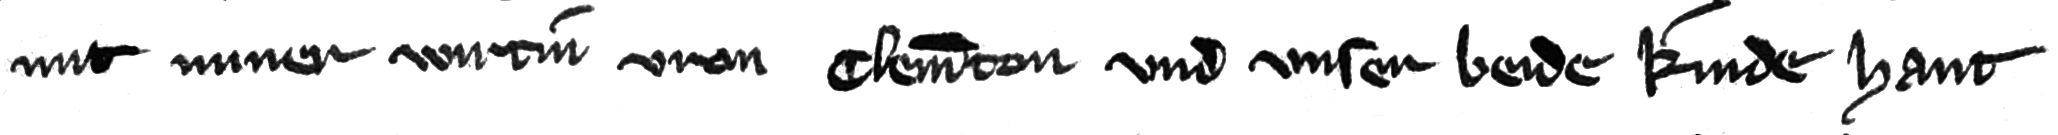
\includegraphics[
	width=\linewidth,
]{./figures/CAO_01843_ausschnitt.jpg}
\caption%
	[Ausschnitt aus Bern, Staatsarchiv, StABE~C~I~a, Stift 1293.11.30]%
	{Ausschnitt aus Bern, Staatsarchiv, StABE~C~I~a, Stift 1293.11.30
		\autocites(Foto: Staatsarchiv Bern)[\pno~1843]{cao3}}
\label{fig:1843}
\end{figure}

Der einzige weitere Beleg in einem ähnlichen syntaktischen Kontext wird in
\cref{ex:682_insigel} zitiert. Hier urkunden Abt Volland und Prior Berthold
gemeinsam mit der Klostergemeinschaft. Die Form \lit{bediu} lässt auf Kongruenz
mit \lit{inſigel} `Siegel' schließen. Der Beleg wurde aufgrund des Hiatus
nicht in \cref{tab:caosimprefctrl} aufgenommen.

\begin{exe}
\ex\label{ex:682_insigel}
	% https://www.wubonline.de/?wub=4267
	% Stuttgart, Hauptstaatsarchiv, A 514 U 50
	\gll Tougen wir abt vollant / vnd Bertholt der prior / vnd der Conuent von
			Hirſowe kunt \textelp{} {dar umbe} haben\footnotemark{}
			wir an dizen breif vnſer bediu inſigel / vnd Grauen
			Aberetheſ von · hohenberc \\
		tun wir Abt Volland[\Nom.\Sg.\MascM] {} und Berthold[\Nom.\Sg.\MascM]
			der Prior {} und der Konvent[\Nom.\Sg.\M\subM] von Hirsau kund {}
			Darum heben \Fpl\subM.\Nom{} an diesen Urkunde
			\Fpl.\Gen.\Pl\subM{} beide-\Acc.\Pl.\NeutI.\St{}
			Siegel[\Acc.\Pl.\NeutI] {} und Graf-\Gen.\Sg{} Albrecht-\Gen{} von
			{} Hohenberg \\
		\trans `machen wir, Abt Volland und Berthold der Prior und der
			Konvent von Hirsau bekannt \textelp{} darum hängen wir an diese
			Urkunde unsere beiden Siegel und Graf Albrechts von
			Hohenberg'
			\parencites(Nr.~682, Kl.~Hirsau, Kr.~Calw, 1284)[96,3 und 11--12]{cao2}
		%
		\footnotetext{Das \citet[780]{wmu1} vermerkt eine
			\textquote{\textins*{g}elegentl.\ Vermengung der Formen von
			\emph{haben} und \emph{heben}}, die auch an dieser Stelle
			anzunehmen ist.}
\end{exe}

Im \REM{} finden sich zum Vergleich noch zwei Belege mit \norm{bėide} aus
dem mitteldeutschen Sprachraum, der bei der vorliegenden Untersuchung
ausgeklammert wurde. Die Belege werden in \cref{ex:remgenbeide} zitiert. Die
Annotation ist aus dem \REM{} übernommen und in \cref{ex:remgenbeide_1}
unklar. Belege für \norm{bėidiu} im Gen.\ Pl.\ konnten nicht gefunden werden,
das heißt, \lit{-í} in \lit{beidí} ist in \cref{ex:remgenbeide_1} nicht
als Variante von \norm{-iu} zu werten, sondern als ostmitteldeutsche
Schreibweise für \norm{-e} \autocites[52--53]{paul2007}[305]{ksw2}.%
%
	\footnote{
		\begin{tabularx}{\linewidth}[t]{@{} l @{~=~} l @{}}
		M320 &
			\tit{Mühlhäuser Rechtsbuch}
			(Nordhausen, Stadtarchiv, Ms. II, Na 6; \cite[1379]{hsc});
		\\

		M350 & Köln, Historisches Archiv der Stadt, Best.~210 (Domstift), U~3/759 (\DTMdate{1306-09-01}).
		\\
		\end{tabularx}
	}

\begin{exe}
\ex \label{ex:remgenbeide}
\begin{xlist}
	\ex \label{ex:remgenbeide_1}
		\gll von den luitín die vrí beidí gívoren ſien \\
			von den Leuten die ihr-\Gen.\Pl{} beide-\Gen.\Pl{}
			\tsup{?}\norm{gevuore}-\Nom.\Pl.\MascA{} sind
			\\
		\trans `von den Leuten, die ihr beider Fahrtgenossen (?) sind'
			% M320 = 'Mühlhäuser Rechtsbuch' (Nordhausen, Stadtarchiv, Ms. II,
			% Na 6; HSC 1379)
			\parencite[M320: 17v,21--22]{rem}

	\ex \label{ex:remgenbeide_2}
		\gll van dode der kindˢe beide of irre eyn \\
			von Tod-\Dat.\Sg{} der Kind-\Gen.\Pl{} beide-\Gen.\Pl.\St{} oder
			ihrer ein \\
		\begin{taggedline}{\parencite[\nopp{}M350, 5, 11]{rem}}
		\trans `durch den Tod beider Kinder oder eines von ihnen'
		\end{taggedline}
\end{xlist}
\end{exe}

\paragraph{Unbelebt, gleiches Genus}

Bei Belegen für \norm{bėide} mit indirektem Bezug auf unbelebte kombinierte
Erstcontroller mit gleichem Genus ergibt sich in \cref{tab:caosimprefctrl} ein
Spiegelbild zum belebten Gegenstück. Neben 23 Fällen von \norm{bėidiu} mit
neutralem Bezug ist die neutrale Form auch in vier von sechs Fällen mit
kombiniertem maskulinem Bezug zu finden \cref{ex:cao_samegend_inan_mm_beidiu}.
Belege für die Kombination zweier unbelebter Feminina sind im ausgewerteten
Material keine vorhanden.

\begin{exe}
\ex \label{ex:cao_samegend_inan_mm_beidiu}
	\begin{xlist}
	\ex \label{ex:cao_samegend_inan_mm_beidiu_1}
		\gll vnſerne zehenden zeandeluingen vnde ainen Garten
				\textelp{} div wier baidiv fvr reht aigen her
				haigen~\textins{sic} braht \\
			unseren Zehnt-\Acc.\Sg{}.\MascI{} zu=Andelfingen und einen
				Garten-\Acc.\Sg.\MascI{} {} \Rel.\Acc.\Pl.\NeutI{} wir
				beide-\Acc.\Pl{}.\NeutI.\St{} für rechtmäßig Eigentum her haben
				gebracht \\
		\trans `unseren Zehnten zu Andelfingen und einen Garten \textelp{},
			die wir beide als recht\-mäßiges Eigentum hergebracht haben'
			\parencites(Nr.~1201~AB, Kl.~Heiligkreuztal, Kr.~Biberach, 1290)[472,10--18]{cao2}

	\ex \label{ex:cao_samegend_inan_mm_beidiu_2}
		\gll Einen garten vnde einen aker {}
				ligent beidú bi \textelp{} Mit allem dem rehte alſ er
				{-- --} ſú bedú von mir hatte \\
			einen Garten-\Acc.\Sg.\MascI{} und einen Acker[\Acc.\Sg.\MascI]
				Ø liegen beide-\Nom.\Pl.\NeutI.\St{} bei {} mit allem dem
				Recht als er {} \Tpl.\Acc{} beide-\Acc.\Pl.\NeutI.\St{} von mir
				hatte \\
		\trans `einen Garten und einen Acker, \textins{die} liegen beide
			bei \textelp{}, mit all dem Recht, wie er sie beide von mir hatte'
			\parencites(Nr.~3249, Freiburg i.\,Br., 1299)[417,4--6]{cao4}
	\end{xlist}
\end{exe}

Der Beleg in \cref{ex:cao_samegend_inan_mm_beidiu_1} -- bis auf kleine
Unterschiede in der Großschreibung sind beide Fassungen identisch -- scheint
auf den ersten Blick ambig bezüglich des Antezedens von \lit{baidiv} zu sein.
Allerdings kann die Lesart mit \lit{wier baidiv} `wir beide' als Einheit
im Kontext der Urkunde ausgeschlossen werden, da drei Aussteller genannt
werden: die Brüder \lit{wezel vn̄ hainrich wezel vnde Cvͦnrat der Bodemer}
% `Wezel und Heinrich Wezel und Konrad der Bodemer'
\autocite[\pno~1201~AB, 472.7]{cao2}.

Während sich im Material zum \CAO{} keine kombinierten unbelebten
Feminina finden ließen, lieferte eine kurze Recherche im \REM{} die drei
in \cref{ex:beid2p2combrem} zitierten Belege zurück, allerdings stammen zwei
davon aus gereimten Texten.%
%
	\footnote{
		\begin{tabularx}{\linewidth}[t]{@{} l @{~=~} l @{}}
		M317 &
			Hugo von Langenstein: \tit{Martina}
			(Basel, Universitätsbibl.,	Cod. B~VIII~27; \cite[2776]{hsc});
		\\

		M342 &
			Gottfried von Straßburg: \tit{Tristan}
			(München, Bayerische Staatsbibl., Cgm~51; \cite[1286]{hsc});
		\\	

		M401 &
			\tit{Baumgarten geistlicher Herzen}
			(München, Bayerische Staatsbibl., Cgm~6247; \cite[1450]{hsc}).
		\\
		\end{tabularx}

		Die Details zu den exzerpierten Passagen können der Webseite des
		\citet[s.\,u.~detaillierte Textübersicht]{rem} entnommen werden.}
%
Alle drei Belege weisen die neutrale Form \norm{bėidiu} mit Bezug auf
kombinierte unbelebte Feminina auf.

\begin{exe}
\ex \label{ex:beid2p2combrem}
	\begin{xlist}
	\ex \label{ex:beid2p2combrem_1}
		\gll Dˢ ſol dich ſchiere machī bloz \\
			der wird dich sogleich machen nackt \\
	\sn \gll Gewaltis vn̄ der eren \\
			Macht[\Gen.\Sg.\FemI] und der Ruhm[\Gen.\Pl.\FemI] \\
	\sn \gll Div sol er beidiv keren \\
			\Dem.\Acc.\Pl.\NeutI{} wird er beide-\Acc.\Pl.\NeutI.\St{}
			verwandeln \\
	\sn \gll In laſtir menicvalt \\
			in Laster vielfältig \\
		\trans `Der wird dich sogleich entblößen der Macht und des Ruhms.
			Die wird er beide in vielfältige Laster verwandeln.'
			\parencite[M317: V.~13020--13023]{rem}

	\ex \label{ex:beid2p2combrem_2}
		\gll daz triwe vn̄ ere werde. \\
			dass Treue[\Nom.\Sg.\FemI] und Ruhm[\Nom.\Sg.\FemI] werde \\
	\sn \gll begraben in die erde. \\
			begraben in die Erde \\
	\sn \gll ſo ligent ſi beidiv hie begraben. \\
			so liegen \Tpl\subI.\Nom{} beide-\Nom.\Pl.\NeutI.\St{} hier
			begraben \\
		\trans `dass Treue und Ruhm werde / begraben in der Erde. / So
			liegen sie beide hier begraben.'
			\parencite[M342: V.~18661--18663]{rem}

	\ex \label{ex:beid2p2combrem_3}
		\gll der iſt genant ſineſ vater tugent vn̄ wiſheit
			{da von} ſvln ſínív ſchulcheit\upshape\footnotemark{} diſiv
			beidiv von ím lernen. \\
			der ist genannt seines Vater Tugend[\Nom.\Sg.\FemI] und
			Weisheit[\Nom.\Sg.\FemI] davon sollen seine Schulkind
			diese-\Acc.\Pl.\NeutI.\St{} beide-\Acc.\Pl.\NeutI.\St{} von ihm
			lernen \\
		\trans `der wird genannt Tugend und Weisheit seines Vaters.
			Deshalb sollen seine Schulkinder diese beide von ihm lernen.'
			\parencite[M401: 108v,19--21]{rem}
	\end{xlist}
\end{exe}
%
	\footnotetext{Die Schreibung wurde am Digitalisat der Handschrift
%	(\href{https://mdz-nbn-resolving.de/urn:nbn:de:bvb:12-bsb00104263-7}{urn:nbn:de:bvb:12-bsb00104263-7})
	verifiziert, die Glossierung aus dem \REM{} übernommen. Dieselbe
	Textstelle in M405Y (München, Bayerische Staatsbibl., Cgm 183: Bl.~4\vo, 5;
	\cite[9715]{hsc}% ;
% 	\href{https://mdz-nbn-resolving.de/urn:nbn:de:bvb:12-bsb00006141-6}{urn:nbn:de:bvb:12-bsb00006141-6}
	) enthält dafür \lit{ſchvͦl chint} `Schulkinder' und ebenso \lit{diſiv
	beidiv} `diese beide (\N)'.}

\paragraph{Unbelebt, verschiedenes Genus}

Die Belege in \cref{tab:caosimprefctrl} für \norm{bėide}-Targets in
Abhängigkeit von unbelebten Erstcontrollern mit unterschiedlichem Genus
verhalten sich noch regelmäßiger als ihr belebtes Gegenstück. Die Beispiele in
\cref{ex:cao_diffgend_inan} illustrieren den hier diskutierten
Kongruenzkontext.

\begin{exe}
\ex \label{ex:cao_diffgend_inan}
	\begin{xlist}
	\ex \label{ex:cao_diffgend_inan_1}
		\gll daz ich auz minem hauz vnd auz miner hofſtat
			div bediv min recht eigen ſint \\
			dass ich aus meinem Haus[\Dat.\Sg.\NeutI] und aus meiner
			Grundstück[\Dat.\Sg.\FemI] \Rel.\Nom.\Pl.\NeutI{}
			beide-\Nom.\Pl.\NeutI.\St{} mein rechtmäßig Eigentum sind \\
		\trans `dass ich aus meinem Haus und aus meinem Grundstück, die 
			beide mein rechtmäßiges Eigentum sind'
			\parencites(Nr.~1282, Regensburg, 1290)[526,37--38]{cao2}

	\ex \label{ex:cao_diffgend_inan_2}
		\gll an dem hofe da ce Holtzhvſen \textelp{} vnde an der
			holtzmark die ich da han, div baidiv min
			reht aigen waren \\
			an dem Hof-\Dat.\Sg.\MascI{} da zu Holzhausen {} und an der
			Waldstück[\Dat.\Sg.\FemI] \Rel.\Nom.\Sg.\FemI{} ich da habe
			\Rel.\Nom.\Pl.\NeutI{} beide-\Nom.\Pl.\NeutI.\St{} mein
			rechtmäßig Eigentum waren \\
		\trans `an dem Hof in Holzhausen \textelp{} und an dem Waldstück,
			das ich da habe, die beide mein rechtmäßiges Eigentum waren'
			\parencites(Nr.~N~272, Augsburg, 1285)[215,30--31]{cao5}
	\end{xlist}
\end{exe}

In allen sieben Fällen steht eine Form vom Typ \norm{bėidiu}. Sieben Belege
sind nicht genug, um daraus eine Regel abzuleiten, aber die vorhandenen Belege
fügen sich mit denen zum belebten Kontext zu einem Bild zusammen. Insgesamt ist
auffällig, dass nahezu alle Targets mit unbelebter kombinierter Referenz die
neutrale Kongruenzform \norm{bėidiu} aufweisen, unabhängig vom Genus ihrer
Erstcontroller.

\subsubsection{Indirekter Bezug auf unkombinierte Plural-Controller}
\label{subsubsec:beid2p2snglncao}

Zuletzt bleiben noch Belege für Targets zu diskutieren, die sich auf einen
pronominalen Controller beziehen, der sich seinerseits auf ein einzelnes
Substantiv im Plural bezieht. Ein Beispiel für diesen syntaktischen Kontext
gibt \cref{ex:beid2p2snglncao}.

\begin{exe}
\ex \label{ex:beid2p2snglncao}
	\begin{tikzpicture}[baseline=(2_lb1.base)]
	    \node at (0,0)  (1)     [gray]
	                            {\lit{wroͮwen}};
	    \node           (1_box) [draw,gray,rectangle,fit=(1)] {};
	    \node           (1_lb)  [above=.5ex of 1_box, gray, font=\mynodefont]
	                            {Controller};

		\node at (3,0) (2)      {\lit{ſi}};
	    \draw (2) node (2_box1) [
	                        draw,
	                        gray,
	                        minimum height=3em,
	                        minimum width=3em,
	                        xshift=-.5ex,
	                        yshift=+.5ex,
	                        rectangle
	                    ] {};
	    \draw (2) node (2_box2) [
	                        draw,
	                        minimum height=3em,
	                        minimum width=3em,
	                        xshift=+.5ex,
	                        yshift=-.5ex,
	                        rectangle
	                    ] {};
	    \node           (2_lb1) [above=.5ex of 2_box1, gray, font=\mynodefont]
	                            {Target};
	    \node           (2_lb2) [below=.5ex of 2_box2, font=\mynodefont]
	                            {Controller};

	    \node at (6,0)  (3)      {\lit{beide}};
	    \node           (3_box)  [draw,rectangle,fit=(3)] {};
	    \node           (3_lb)   [above=.5ex of 3_box, font=\mynodefont]
	                            {Target};

	    \draw [-latex,gray] (1_box)  to [yshift=-1.5ex]     (2_box1);
	    \draw [latex-]      (3_box)  to [yshift=1.5ex]      (2_box2);
	\end{tikzpicture}

\sn \gll vnd ſol ez den zwein wroͮwen gen biz an ir beider tot / ſo
		ſi beide nit enſint \textelp{} \\
		und soll es den zwei Frauen-\Dat.\Pl.\FemF{} übergeben bis an ihr
		beider Tod {} wenn \Tpl\subF.\Nom{} beide-\Nom.\Pl.\M+\F\subF.\St{}
		nicht \Neg=sind {} \\
	\trans `und soll es den zwei Frauen übergeben bis an ihr beider Tod.
		Wenn sie beide nicht \textins{mehr} sind, \textelp{}'
		\parencites(Nr.~2568, Sirnau, Kr.~Esslingen, 1297)[3,31]{cao4}
\end{exe}

Wie zuvor dienen diese Belege als Vergleich für diejenigen mit Bezug auf
kombinierte Erstcontroller. Ihre Verteilung nach den Personenmerkmalen des
Erstcontrollers gibt \cref{tab:caosimprefctrl2} an. Wie auch in
\cref{tab:simpnomctrl}, dort mit direktem Bezug auf ein Substantiv im Plural,
löst beim indirekten Bezug über ein Pronomen maskuline und feminine Referenz
wie erwartet die Kongruenzform \norm{bėide} aus, neutrale Referenz dagegen eine
Form vom Typ \norm{bėidiu}. Belebtheit scheint auch hier keine Rolle zu
spielen, wenn sich die drei Belege für unbelebte Feminina regelmäßig verhalten.

\begin{table}
\centering
\caption{Flexion nach Personenmerkmalen der anaphorischen Controller
(einfacher Bezug)}
\begin{tabular}{
l
%	@{\hspace{4\tabcolsep}}
	l
    r
    r
    r
}
\toprule
\mc{2}{c}{Controller}
    & bėid(e)
    & bėidiu
    & Summe
    \\
\midrule
% Controller     | e  | iu | Σ
\Tpl & \MascM    &  2 &    &  2 \\
     & \FemF     &  3 &    &  3 \\
     & \NeutF    &    &  4 &  4 \\
     & \NeutX    &    &  2 &  2 \\

\cmidrule{2-5}

     & \FemI     &  3 &    &  3 \\

\midrule

\mc{2}{l}{Summe} &  8 &  6 & 14 \\

\bottomrule
\end{tabular}
\label{tab:caosimprefctrl2}
\end{table}

Im Fall der Formen mit \norm{-iu} unterscheidet \cref{tab:caosimprefctrl2}
zwischen dem Bezug auf Neutra mit weiblichem Bezug und solchen mit unbekanntem
Bezug. Auch wenn die resultierende Kongruenz\-form in beiden Fällen die gleiche
ist, möchte ich die Belege kurz charakterisieren. Die Belege für ersteren
Kontext werden in \cref{ex:cao_beidiu_neutfem} zitiert.

\begin{exe}
\ex \label{ex:cao_beidiu_neutfem}
	\begin{xlist}
	\ex \label{ex:cao_beidiu_neutfem_1}
		\gll engiltrvt ir tohtir Vn̄ annvn ir thohtir thohtir
			\textelp{} ſtirpth der {vor genandon} kint eiz \textelp{}
			ſterbinz {beidiv \textelp{}} \\
			Engeltraut ihr Tochter und Anna-\Obl{} ihr Tochter Tochter {}
			stirbt der vorgenannten Kind[\Gen.\Pl.\NeutF] eines {}
			sterben=\Tpl\subF.\Nom{} beide-\Nom.\Pl.\NeutF.\St{} \\
		\trans `Engeltraut, ihre Tochter, und Anna, ihrer Tochter Tochter
			\textelp{} stirbt der vorgenannten Kinder eines \textelp{}
			Sterben sie beide \textelp{}'
			\parencites(Nr. 629, St.~Gallen, 1284)[57,24--25]{cao2}

	\ex \label{ex:cao_beidiu_neutfem_2}
		\gll Gerhauſe vnde Diemvde \textelp{} vnde ſwenne {der ſelben}
			chinde einz ſtirbet \textelp{} die wile ſi
			beidiv lebent \textelp{} vnde daz der chinde einz
			dannoch lebt oder ſi beidiv \\
			Gerhaus-\Dat.\Sg.\FemF{} und Diemut-\Dat.\Sg.\FemF{} {} und so=wenn
			derselben Kind-\Gen.\Pl.\NeutF{} eines stirbt {} die Weile
			\Tpl\subF.\Nom{} beide-\Nom.\Pl.\NeutF.\St{} leben {} und dass der
			Kind-\Gen.\Pl.\NeutF{} eines {dann noch} lebt oder \Tpl\subF.\Nom{}
			beide-\Nom.\Pl.\NeutF.\St{} \\
		\trans `Gerhaus \textins{sic} und Diemut \textelp{} und wenn
			irgendwann derselben Kinder eines stirbt \textelp{} Während sie
			beide am Leben sind \textelp{} und dass der Kinder eines dann
			noch lebt oder sie beide \textelp{}'
			\parencites(Nr.~2719, Nürnberg, 1297)[96,43--97,9]{cao4}

	\ex \label{ex:cao_beidiu_neutfem_3}
		\gll ſweſter Gerdrauden vnd ſweſter Diemvden hern wernhereſ
			chinden \textelp{} vnd ſwenne der vorbenannten chinde
			einez ſtirbet \textelp{} Di weil ſi peidev
			lebent \\
			Schwester Gertraut[\Dat.\Sg.\FemF] und Schwester
			Diemut[\Dat.\Sg.\FemF] Herrn Wernhers Kinder-\Dat.\Pl.\NeutF{} {}
			und so=wenn der vorbenannten Kind-\Gen.\Pl.\NeutF{} eines stirbt
			{} die Weile \Tpl\subF.\Nom{} beide-\Nom.\Pl.\NeutF.\St{} leben \\
		\trans `Schwester Gertraut und Schwester Diemut, Herrn Wernhers
			Kindern \textelp{} Und wenn irgendwann der vorgenannten Kinder eines
			stirbt \textelp{} Während sie beide am Leben sind'
			\parencites(Nr.~2960, Engelthal, Kr.~Nürnberger Land, 1298)[240,31--38]{cao4}
	\end{xlist}
\end{exe}

Bei allen vier \norm{bėidiu}-Targets geht es um \norm{kint}, also wörtlich
`Kinder', wobei dieser Begriff gemäß \citet[s.\,v.~\fw{kint}]{lexer:mhdhwb}
hier treffender in der Bedeutung `Tochter'
\crefrange{ex:cao_beidiu_neutfem_1}{ex:cao_beidiu_neutfem_3} oder vielleicht
auch spezifischer `Klosterangehörige'
\crefrange{ex:cao_beidiu_neutfem_2}{ex:cao_beidiu_neutfem_3} aufzufassen ist.
Die \norm{kint} sind dabei im Kontext der Rechtssprache nicht zwangsläufig
minderjährig, insofern Erwachsene unabhängig von ihrem Alter Kinder ihrer
Eltern sind \autocites[vgl.][1736]{schwab2012}[siehe
auch][258--259]{birkenesfleischer2022}. Um welche Personen es sich bei den
\norm{kint} jeweils handelt, geht aus dem Kontext der jeweiligen Urkunden
hervor. Bei \cref{ex:cao_beidiu_neutfem_2,ex:cao_beidiu_neutfem_3} handelt es
sich um die gleichen Personen, die Schwestern Gertraut und Diemut, Töchter des
Wernher vom Stein und Mitglieder des Konvents von Engelthal
\autocite[Kr.~Nürnberger Land; vgl.][619]{caor}.
%
Die Kongruenz zwischen \lit{ſi} und \lit{chinde} `Kinder' wurde hier
jeweils aufgrund der Nähe zwischen pronominalem Target und nominalem Controller
angenommen. Im ganzen unter\-suchten Material ließen sich keine Belege für
direkte Kongruenz zwischen \norm{bėidiu} und zwei weiblichen Controllern finden%
% , die eine Hypothese über exophorische Kongruenz ermöglichen würden, für
% \norm{bėide} allerdings auch nicht
. Eine Recherche diesbezüglich im
\REM{} lieferte keine Ergeb\-nisse.
% , allerdings sind dessen Suchfunktionen zum gegenwärtigen Zeitpunkt nicht
% darauf ausgelegt, komplexe syntaktische Kontexte zu durchsuchen.

Den Beispielen in \cref{ex:cao_beidiu_neutfem} steht der Beleg in
\cref{ex:cao_beidiu_neutunkn} gegenüber. In dieser Urkunde werden die Kinder
nicht beim Namen genannt, allerdings geht der Umstand aus dem Text hervor, dass
zumindest eines von ihnen noch nicht \lit{ze ſinen tagen} `zu seinen
Tagen' \autocites[\pno~214, 218.18--19]{cao1}[vgl.][26]{caor} gekommen, also
minderjährig ist. Auch hier wurde Kongruenz nach der Form zwischen
\lit{kinden} `Kindern' und \lit{ſvͥ beidvͥ} angenommen.

\begin{exe}
\ex \label{ex:cao_beidiu_neutunkn}
	\gll mit zewain kinden \textelp{} daz ſvn ſvͥ
		beidvͥ han vnze an ir tôt \textelp{} vn̄ ſwen
		ſvͥ beidvͥ {en ſîn}
		\textelp{} \\
		mit zwei Kind-\Dat.\Pl.\NeutX{} {} das sollen
		\Tpl\tsub{\SX}.\Nom{} beide-\Nom.\Pl.\NeutX.\St{} haben bis an ihr
		Tod {} und so=wenn \Tpl\tsub{\SX}.\Nom{}
		beide-\Nom.\Pl.\NeutX.\St{} \Neg=sind {} \\
	\trans `mit zwei Kindern \textelp{} das sollen sie beide besitzen
		bis an ihren Tod \textelp{} Und wenn sie beide irgendwann nicht
		\textins{mehr} sind \textelp{}'
		\parencites(Nr.~214, Rottweil, 1274)[218.17--24]{cao1}
\end{exe}

\subsubsection[Zu Askedals (1973) Hypothese der ‚Monoflexion‘]{Zu \posscite{askedal1973} Hypothese der \q*{Monoflexion}}
\label{subsubsec:monoflexioncao}

\citet[99]{askedal1973} stellt bezüglich der Konstruktion `sie beide' eine
Hypothese zur \q*{Monoflexion} auf. Diese besagt, dass nur eines der beiden
Glieder neutral flektiert würde. Er schließt dies aus der Häufigkeit der Belege
für \norm{die/-iu beide} beziehungsweise \norm{si beide/-iu} in seiner
Stichprobe aus der \citetitle{maroldschroeder1969}-Edition von
\citet{maroldschroeder1969} und der Edition des \citetitle{lachmannhartl1952}
von \citet{lachmannhartl1952}. \cref{tab:asksiebeidekombis} gibt die Ergebnisse
der Auswertung von \citet{askedal1973} wieder; bei den Zahlen in Klammern
\blockcquote[99]{askedal1973}{sind die wahrscheinlichen Elisionsformen mit
einbegriffen}, also Kontexte, in denen der Vokal des Flexionssuffixes im
Hiatus oder am Zeilenende steht.

\begin{table}
\centering
\caption{Kombinationen von \norm{si} und \norm{die/diu} mit \norm{bėide/-iu} \parencite[99]{askedal1973}}
\begin{tabular}{
	l
	r r
	r
	@{\hspace{4\tabcolsep}}
	r r
}
\toprule
Controller
	& \mc{2}{c}{bėide}
	& bėidiu
	& \mc{2}{c}{Summe}
	\\

\midrule

%     | e         | iu | Σ         |
si    &  7 & (14) &  6 & 13 & (20) \\

\midrule

die   &  0 &  (1) &    &  0 &  (1) \\
diu   & \mc{2}{c}{1} &    & \mc{2}{c}{1} \\

\midrule

Summe &  8 & (16) &  6 & 14 & (22) \\
\bottomrule
\end{tabular}
\label{tab:asksiebeidekombis}
\end{table}

In einer Teilauswertung des \CAO{} konnte festgestellt werden, dass in
der Tat \norm{si} die häufigste Form des Pronomens der 3.\ Pers.\ Nom./Akk.\
Pl.\ darstellt. Dies dürfte jedoch weniger der Vermeidung von Redundanz in der
Markierung als vielmehr der Tatsache geschuldet sein, dass sich Ende des
13.~Jahrhunderts der Typ \norm{si} ohne Genusdistinktion als die geläufige
oberdeutsche Form dieses Pronomens etabliert hat. \citet[392, Abb.~P~26]{ksw2} verzeichnen in der zweiten Hälfte des 13.\ Jahrhunderts
für das Bairische, den alemannisch-bairischen Übergangsbereich und das
Alemannische Werte zwischen 96 und 100\,\% für diesen Typ. Die
\cref{tab:caosiebeidekombis} zeigt die im \CAO{}-Material belegten
Kombinationen und ihre Häufigkeit.

\begin{table}
\centering
\caption{Kombinationen von \norm{si/sie/siu} und \norm{di/die/diu} mit \norm{bėide/-iu} im
\CAO{}}
\begin{tabular}{
	l
	r r
	r
}
\toprule
Controller
	& bėid(e)
	& bėidiu
	& Summe
	\\

\midrule

%     | e  | iu | Σ  |
si    &  8 & 19 & 27 \\
sie   &  3 &  3 &  6 \\
siu   &  5 &  9 & 14 \\

\midrule

di    &  1 &    &  1 \\
die   &  3 &    &  3 \\
diu   &    &  4 &  4 \\

\midrule

Summe & 20 & 35 & 55 \\
\bottomrule
\end{tabular}
\label{tab:caosiebeidekombis}
\end{table}

Eine klare Präferenz für bestimmte Kombinationen ist aus den Daten in
\cref{tab:caosiebeidekombis} nicht herauszulesen. Es bleibt höchstens darauf
hinzuweisen, dass sowohl \norm{sie bėidiu}
% \cref{ex:siebeidiu}
als auch \norm{siu bėide}
%\cref{ex:siubeide}
mehrmals belegt sind. Bei \norm{sie bėidiu} stammen zwei Belege aus dem
bairischen Sprachraum (Rothenburg ob der Tauber, Kloster Stams) und einer aus
dem schwäbischen (Kloster Heiligkreuztal); bei \norm{siu bėide} fanden sich
alle fünf Belege in alemannischen Urkunden (Kloster Kirchberg, Überlingen,
Zürich). Da in keiner der Urkunden, die diese Belege enthalten, ein
systematischer Unterschied zwischen \norm{si}, \norm{sie} und
\norm{siu} festgestellt werden konnte, müssen sie als zum genusneutralen Typ
\norm{si} gehörig gewertet werden.

% \begin{exe}
% \ex \label{ex:siebeidiu}
% 	\gll Otto der Crvͤcær / vn̄ willebirk ſin hvſvrowe \textelp{} die
% 		wile ſie baidiv lebent \\
% 		Otto[\Nom.\Sg.\MascM] der Kreuzer {} und Wilbirg sein Ehefrau {} die
% 		Weile \Tpl\subMF.\Nom{} beide-\Nom.\Pl.\NeutMF.\St{} leben \\
% 	\begin{taggedline}{\autocite[\pno~636, 64.26]{cao2}}
% 	\trans `Otto der Kreuzer und Wilbirg, seine Ehefrau \textelp{} während
% 		sie beide am Leben sind'
% 	\end{taggedline}

% \ex \label{ex:siubeide}
% \begin{xlist}
% 	\ex \label{ex:siubeide_1}
% 		\gll ... \\
% 			... \\
% 		\begin{taggedline}{\autocite[\pno~1414, 623.26]{cao2}}
% 		\trans \wdef{...}
% 		\end{taggedline}

% 	\ex \label{ex:siubeide_2}
% 		\gll ... \\
% 			... \\
% 		\begin{taggedline}{\autocite[\pno~1504, 679.13]{cao2}}
% 		\trans \wdef{...}
% 		\end{taggedline}
% \end{xlist}
% \end{exe}

Die Belege für \norm{di(e) bėide} und \norm{diu bėidiu} verhalten sich wie
erwartet. Im ersten Fall beziehen sie sich auf Paare aus zwei Männern oder zwei
Frauen, im zweiten auf Paare aus Mann und Frau oder unbelebte Dinge (vgl.
\cref{subsubsec:beid2p2coordncao}).

% \begin{exe}
% \ex \label{ex:diubeidiu}
% 	\begin{xlist}
% 	\ex \label{ex:diubeidiu_1}
% 		\gll ... \\
% 			... \\
% 		\begin{taggedline}{\parencite[\pno~1898, 177.30]{cao3}}
% 		\trans \wdef{}
% 		\end{taggedline}

% 	\ex \label{ex:diubeidiu_2}
% 		\gll ... \\
% 			... \\
% 		\begin{taggedline}{\parencite[\pno~3261, 424.39]{cao4}}
% 		\trans \wdef{}
% 		\end{taggedline}
% 	\end{xlist}
% \end{exe}

\subsubsection{Zusammenfassung und Vergleich}
\label{subsubsec:anaperssum}

Der weitaus größere Teil der Urkundenbelege für \norm{bėide} entfällt auf
Targets mit pro\-nomi\-nalem Controller und damit auf eine bloß indirekte
Abhängigkeit von kombinierten Controllern. Dies bedeutet jedoch nicht, dass
entsprechende weitere Untersuchungen für diesen syntaktischen Zusammenhang
nicht relevant wären, da auch auf Distanz Variation in der Genusmarkierung von
\norm{bėide} als indirektes Target zweier NPs beobachtet werden kann. 
Es konnte nicht festgestellt werden, dass Pronomen, die nicht
nach Genus flektieren, einen neutralisierenden Effekt auf die Form von
\norm{bėide} haben, insofern dass danach immer entweder \norm{bėide} oder \norm{bėidiu} stehen würde.
% Dies lässt sich dadurch begründen, dass auch bei Pronomen ohne morphologische
% Genusmarkierung (\norm{ich}, \norm{wir}, \norm{uns}, \norm{si}, \norm{di})
% auf semantischer Ebene die Koindizierung mit Substantiven steht.

\Cref{tab:cao_e_iu_coord} fasst die Verteilung der Belege für \norm{bėide}
aus \cref{tab:combnomctrl,tab:caosimprefctrl} noch einmal vereinfacht zusammen.
Insgesamt scheint bei der Kongruenzbeziehung zwischen zwei Controllern und
\norm{bėide} ($N_i + N_j$) die Belebtheit der Substantive eine wichtigere
Rolle als deren Genus zu spielen. Aufgrund der geringen Zahl der Belege für den
direkten Bezug auf kombinierte Controller wurden hier die in
\cref{tab:combnomctrl} grau gedruckten Belege mitgezählt, da sie sich nicht
anders verhalten als ihre regulär gezählten Gegenstücke. Aussagen über das
Verhalten des Targets beim direkten Bezug von \norm{bėide} auf zwei unbelebte
Substantive können keine gemacht werden, da dieser Kontext in der Stichprobe
nicht belegt ist.

\begin{table}
\centering
\caption{Flexion nach syntaktischem Kontext (kombinierter Bezug)}
\begin{tabular}{
	l l
	c
	r r
	c
	r r
	c
	r
}
\toprule
\mr{2}{*}{Belebtheit}
	& \mr{2}{*}{Geschlecht}
	& %
	& \mc{2}{c}{$N_i + N_j$}
	& %
	& \mc{2}{c}{$PRO_{i + j}$}
	& %
	& \mr{2}{*}{Summe}
	\\

\cmidrule{4-5}
\cmidrule{7-8}

%
	& %
	& %
	& bėid(e)
	& bėidiu
	& %
	& bėid(e)
	& bėidiu
	& %
	& %
	\\

\midrule

belebt
	& gleich
	& %
	&   1
	&   1
	& %
	&  16
	& 
	& %
	&  18
	\\

%
	& verschieden
	& %
	& 
	&   2
	& %
	&  17
	&  47
	& %
	&  66
	\\

\midrule

unbelebt
	& gleich
	& %
	& 
	&   1
	& %
	&   2
	&  27
	& %
	&  30
	\\

%
	& verschieden
	& %
	& 
	& 
	& %
	& 
	&   7
	& %
	&   7
	\\

\midrule

\mc{2}{l}{Summe}
	& %
	&   1
	&   4
	& %
	&  35
	&  81
	& %
	& 121
	\\

\bottomrule
\end{tabular}
\label{tab:cao_e_iu_coord}
\end{table}

Beim direkten Bezug auf zwei belebte Controller mit verschiedenem Sexus ist nur
\norm{bėidiu} belegt, allerdings mit zwei Belegen nicht sehr häufig. Wesentlich
besser belegt ist der indirekte Bezug von \norm{bėide} auf zwei Erstcontroller
mittels eines Pronomens ($PRO_{i+j}$). Hier liegen für den indirekten Bezug auf
zwei belebte Erstcontroller von gleichem Geschlecht ausschließlich Belege für
\norm{bėide} vor. Beim indirekten Bezug auf zwei belebte Substantive von
unterschiedlichem Geschlecht tritt dagegen Variation zwischen \norm{bėide} und
\norm{bėidiu} auf, wobei die neutrale Form \norm{bėidiu} mehr als doppelt so
häufig vertreten ist.

Beim indirekten Bezug auf kombinierte unbelebte Erstcontroller vom gleichen
Genus entfällt der Großteil der Belege auf \norm{bėidiu} und lediglich zwei auf
\norm{bėide}. Im Fall des indirekten Bezugs auf zwei unbelebte Substantive von
unterschiedlichem Geschlecht ist nur die Form \norm{bėidiu} belegt. Insgesamt
scheint in diesem Kontext also die Form \norm{bėidiu} unabhängig vom Genus
bevorzugt zu werden.

Die Beleglage für den direkten Bezug auf einzelne Plural-Controller wird in
\cref{tab:cao_e_iu_simp} vereinfacht dargestellt, als Quelle dienen die Daten
aus den \cref{tab:simpnomctrl,tab:caosimprefctrl2}. Der Vergleichbarkeit mit
\cref{tab:cao_e_iu_coord} halber wurde auch hier zunächst nach Belebtheit
unterschieden. Die Genera der einzelnen Controller werden jeweils einzeln
aufgeführt, da hier keine Genus-Kombinationen vorliegen. Bei weitem nicht alle
Felder können mit den Belegen aus dem Material des \CAO{} gefüllt
werden. Aufgrund der Lücken lassen sich mit dieser Tabelle allein keine
generellen Aussagen zur Verteilung der \norm{bėide}-Formen mit direktem und
indirekten Bezug auf einzelne Plural-Controller ($N_i$) machen. Die
ausgefüllten Stellen stimmen aber mit dem überein, was nach
\cref{sec:adjdeclcao} regelmäßig zu erwarten ist: Formen vom Typ \norm{bėide}
beschränken sich hauptsächlich auf Kon\-texte mit Bezug auf Maskulina und
Feminina; \norm{bėidiu} ist auf den neutralen Bezug beschränkt. Dies scheint
unabhängig von der Belebtheit und vom syntaktischen Kontext zu gelten.

\begin{table}
\centering
\caption{Flexion nach syntaktischem Kontext (einfacher Bezug)}
\begin{tabular}{
	l l
	c
	r r
	c
	r r
	c
	r
}
\toprule
\mr{2}{*}{Belebtheit}
	& \mr{2}{*}{Genus}
	& %
	& \mc{2}{c}{$N_i$}
	& %
	& \mc{2}{c}{$PRO_i$}
	& %
	& \mr{2}{*}{Summe}
	\\

\cmidrule{4-5}
\cmidrule{7-8}

%
	& %
	& %
	& bėid(e)
	& bėidiu
	& %
	& bėid(e)
	& bėidiu
	& %
	& %
	\\

\midrule

belebt
	& maskulin
	& %
	& 21
	& 
	& %
	&  2
	& 
	& %
	& 23
	\\

%
	& feminin
	& %
	& 
	& 
	& %
	&  3
	& 
	& %
	&  3
	\\

%
	& neutral
	& %
	& 
	& 
	& %
	& 
	&  6
	& %
	&  6
	\\

\midrule

unbelebt
	& maskulin
	& %
	&  7
	& 
	& %
	& 
	& 
	& %
	&  7
	\\

%
	& feminin
	& %
	& 
	& 
	& %
	&  3
	& 
	& %
	&  3
	\\

%
	& neutral
	& %
	&  1
	&  5
	& %
	& 
	& 
	& %
	&  6
	\\

\midrule

\mc{2}{l}{Summe}
	& %
	& 29
	&  5
	& %
	&  8
	&  6
	& %
	& 48
	\\

\bottomrule
\end{tabular}
\label{tab:cao_e_iu_simp}
\end{table}

Beim lexikalischen Blick auf die Kombination \norm{si bėide} hat sich ergeben,
dass -- wie von \citet{askedal1973} für die jeweils verwendeten kritischen
Ausgaben des \tit{Parzival} und des \tit{Tristan} beobachtet -- auch im
\CAO{} mit Abstand die häufigste Variante \norm{si bėide/-iu} ist.
\citeauthor{askedal1973} nimmt an, dass das Fehlen der morphologischen
Markierung von Genus an einem der beiden Glieder grammatikalisiert ist. Eine
Abhängigkeit der Kongruenzform von \norm{bėide} von der Wortform des pronominalen
Controllers konnte im vorliegenden Material jedoch nicht festgestellt werden.
Das umfangreichere Material des \CAO{} weist darüber hinaus mehr
Variation auf als die sehr kleine Stichprobe von \citeauthor{askedal1973}. Die
Häufigkeit von \norm{si} `sie' ist zumindest im \CAO{} der
Vereinfachung des pronominalen Paradigmas hin zu einer genusübergreifenden
Pluralform zuzuschreiben, die nach \citet[391--392]{ksw2} im Oberdeutschen der
zweiten Hälfte des 13.~Jahrhunderts den Normalfall darstellt \autocite[vgl.\
auch][37--39]{sparmann1961}.

%%%%%%%%%%%%%%%%%%%%%%%%%%%%%%%%%%%%%%%%%%%%%%%%%%%%%%%%%%%%%%%%%%%%%%%%%%%%%%%

\section{Targets nach Distanz zum Controller}
\label{sec:caotargdist}

Die Untersuchungen von \citet{corbett1979} zeigen, dass mit zunehmender Distanz
zwischen Controller und Target die Wahrscheinlichkeit für das Auftreten von
Kongruenz \fw{ad sensum} steigt. Die Distanz lässt sich auf zweierlei Arten
messen: zum einen als linearer Abstand in Wortformen (im Sinne von in sich
geschlossenen morphosyntaktischen Einheiten, vgl.~\cite[252--253]{bauer2000}),
zum anderen als syntaktischer Abstand hinsichtlich der Domäne von Target und
Controller (gleiches Satzglied, gleicher Teilsatz, anderer (Teil-)Satz;
vgl.~\cref{sec:ctrltarg}). Die Beispiele in \cref{fig:caodirdist} verdeutlichen
die jeweilige Zählweise.

\begin{figure}
\centering
\subfloat[Abstand nach Wortformen]{%
	\begin{tikzpicture}[
		baseline=(a.base),
		word/.style={
			draw,
			minimum height=1.5em,
			minimum width=4em,
			font=\itshape
		},
		lbl/.style={
			minimum height=1.5em,
			font={\mynodefont}
		},
		every node/.style={
			anchor=base,
			text height=1.5ex,
			text depth=.5ex
		}
	]

	\node [word]                      (1) {Ich};
	\node [word, base right=1ex of 1] (2) {unde};
	\node [word, base right=1ex of 2] (3) {mīn};
	\node [word, base right=1ex of 3] (4) {hūsvrouwe};
	\node [word, base right=1ex of 4] (5) {verjęhen};
	\node [word, base right=1ex of 5] (6) {bėidiu};

	\path[-]      (1) edge [out=north, in=north] node (a) [lbl, above] {0} (2);
	\path[-]      (2) edge [out=north, in=north] node [lbl, above] {1} (3);
	\path[-]      (3) edge [out=north, in=north] node [lbl, above] {2} (4);
	\path[-]      (4) edge [out=north, in=north] node [lbl, above] {3} (5);
	\path[-latex] (5) edge [out=north, in=north] node [lbl, above] {4} (6);
	\path[-]      (4) edge [out=south, in=south] node [lbl, below] {0} (5);
	\path[-latex] (5) edge [out=south, in=south] node [lbl, below] {1} (6);
	\end{tikzpicture}
	\label{fig:caodirdist_words}
}

\subfloat[Abstand nach der syntaktischen Domäne]{%
 	\begin{tikzpicture}[
		baseline=(vflbl.base),
		box/.style={
			draw,
			minimum height=2.5em,
			font=\itshape
		},
		wordbox/.style={
			draw,
			minimum height=1.75em,
			font=\itshape
		},
		lbl/.style={
			minimum height=1.5em,
			font={\mynodefont}
		},
		every node/.style={
			anchor=base,
			text height=1.5ex,
			text depth=.5ex
		}
	]

	\node [wordbox,                    ] (1) {Ich};
	\node [wordbox, base right=1ex of 1] (2) {unde};
	\node [wordbox, base right=1ex of 2] (3) {mīn};
	\node [wordbox, base right=1ex of 3] (4) {hūsvrouwe};
	\node [wordbox, base right=3ex of 4] (5) {verjęhen};
	\node [wordbox, base right=3ex of 5, thick] (6) {bėidiu};
	\node [         base right=3ex of 6] (7) {\phantom{abcdef}};

	\node (VF)  [box, rectangle, fit={(1) (2) (3) (4)}, thick] {};
	\node (LSK) [box, rectangle, fit=(5)] {};
	\node (MF)  [box, rectangle, fit=(6)] {};
	\node (RSK) [box, rectangle, fit=(7)] {};

	\node (vflbl)  [lbl, above=.5ex of VF]  {VF};
	\node (lsklbl) [lbl, above=.5ex of LSK] {LSK};
	\node (mflbl)  [lbl, above=.5ex of MF]  {MF};
	\node (rsklbl) [lbl, above=.5ex of RSK] {RSK};

	\draw [-, thick] (VF) -- ++(south:2em) -| (6);
	\end{tikzpicture}
	\vspace{.5\baselineskip}
	\label{fig:caodirdist_syn}
}
\caption{Zählweisen bei der Abstandsberechnung}
\label{fig:caodirdist}
\end{figure}

In \cref{fig:caodirdist_words} wird der Abstand zwischen den beiden Controllern
\norm{ich} und \norm{(mīn) hūsvrouwe} `(meine) Ehefrau' zu ihrem Target
\norm{bėidiu} `beide' nach Wortformen gezählt. Der erste Sprung zur jeweils
nächsten Wortform wird mit null angesetzt, da zwischen \norm{ich} und
\norm{unde} `und' sowie zwischen \norm{hūsvrouwe} `Ehefrau' und
\norm{verjęhen} `aussagen, bekennen' jeweils kein Abstand besteht. Auf
diese Weise ergibt sich für das Beispiel insgesamt ein kombinierter Wortformenabstand von vier und
eins zwischen Controller und Target.

Bei den Untersuchungen zum Belegmaterial des \CAO{} hat sich die
Entfernungsbestimmung nach Satzgliedern und Sätzen (im Folgenden vereinfachend:
syntaktische Distanz) allerdings als sinnvoller erwiesen. In
\cref{fig:caodirdist_syn} wird das Beispiel der Anschaulichkeit halber
vereinfacht im Rahmen des Feldermodells des deutschen Satzes
\autocites{drach1963}{woellstein2010}[vgl.\ auch][43--51]{mueller2020}
wiederholt. Die Controller \norm{ich} und \norm{hūsvrouwe} `Ehefrau'
stehen im Vorfeld (VF), während das Target \norm{bėidiu} `beide' nach der
linken Satzklammer (LSK) im Mittelfeld (MF) steht. Damit steht das Target in
einem anderen Satzteil als seine Controller, dennoch aber im gleichen Teilsatz,
in diesem Fall dem Hauptsatz (\norm{verjęhen} `aussagen, bekennen' nimmt
in der Regel einen Nebensatz als Komplement). Da die linke Satzklammer mit
einem Vollverb besetzt ist, ist die rechte Satzklammer (RSK) leer. Der
Wortformenabstand steigt tendenziell mit zunehmendem Abstand zwischen
Satzgliedern zueinander und darüber hinaus.

\subsection{Nominale Controller}
\label{subsec:caodistnomctrl}

Für die syntaktische Distanz liegt die in \cref{tab:caocodistp} gezeigte
Belegverteilung vor. Hierbei ist keine Variation in der Lokalität zwischen
beiden Controllern zu beobachten. Es liegen also keine Fälle vor, in denen
beide Controller in unterschiedlichen (Teil-)Sätzen stehen. Aufgrund der
geringen Belegmenge sind auch hier keine starken Konzentrationen von Belegen zu
beobachten. Die unter Vorbehalt aufgenommenen Belege sind grau gedruckt; bei
ihnen handelt es sich in allen Fällen zufällig um Targets in Distanzstellung zu
ihrem Controller (vgl.~\cref{sec:floatquant} zu Floating Quantifiers). In allen
Fällen folgt das Target seinen Controllern.

\begin{table}
\centering
\caption{Flexion nach Distanz von kombinierten nominalen Controllern}
\begin{tabular}{
	l
	c l l
	r
	r
	r
}
\toprule

Domäne
	& Wortdist.
	& Controller 1
	& Controller 2
	& bėide
	& bėidiu
	& Summe
	\\

\midrule

gl.~Satzteil
	& 3 / 0
	& \Tsg.\MascM
	& \Tsg.\FemF
	& %
	& 1
	& 1
	\\

\cmidrule{2-7}

%
	& 7 / 2
	& \Tsg.\MascM
	& \Tsg.\MascM
	& %
	& 1
	& 1
	\\

\midrule

\mc{4}{l}{Summe}
	& 
	& 2
	& 2
	\\

\midrule
\midrule

\gr{gl. Teilsatz}
	& \gr{9 / 3}
	& \gr{\Fsg\subM}
	& \gr{\Tsg.\FemF}
	& %
	& \gr{1}
	& \gr{1}
	\\

\cmidrule{2-7}

%
	& \gr{9 / 4}
	& \gr{\Fsg\subM}
	& \gr{\Fsg\subM}
	& \gr{1}
	& %
	& \gr{1}
	\\

\midrule

\gr{anderer (Teil-)Satz}
	& \gr{20 / 3}
	& \gr{\Tsg.\MascI}
	& \gr{\Tsg.\MascI}
	& %
	& \gr{1}
	& \gr{1}
	\\

\midrule

\mc{4}{l}{\gr{Summe}}
	& \gr{1}
	& \gr{2}
	& \gr{3}
	\\

\bottomrule
\end{tabular}
\label{tab:caocodistp}
\end{table}

Trotz der geringen Belegmenge lässt die Verteilung vermuten, dass
Personenmerkmale eine wichtigere Rolle spielen als die syntaktische Distanz
oder die Distanz nach Wortformen. Einzig der Beleg für zwei unbelebte Maskulina
mit Abstand zwanzig und drei Wortformen fällt durch die unerwartete
\norm{bėidiu}-Form auf. In \cref{subsubsec:beid2p2coordncao} bezüglich des
indirekten Bezugs auf kombinierte Controller konnte jedoch beobachtet werden,
dass bei unbelebtem Bezug häufig auch unab\-hängig vom Genus der Referenten
\norm{bėidiu} steht. Der betreffende Beleg wird in \cref{ex:n241_hofzehnt}
zitiert.

\begin{exe}
\ex\label{ex:n241_hofzehnt}
	\setlength{\glossglue}{5pt plus 2pt minus 1pt}
	\gll daz ich minen frowen von ſande Katerinen minen hof, den ich
		ze Jnningen hete, da etwenne der alte Stevdler ovf ſaz, verkaufft han
		mit dem zehenden, der drovz gat, beidev
		vnuerſchaidenlichen fvͤr reht aigen \\		
		dass ich meinen Frauen von Sankt Katharinen meinen Hof[\Acc.\Sg.\MascI]
		den ich zu Inningen hatte wo vormals der alte Steudler auf saß verkauft
		habe mit dem Zehnt-\Dat.\Sg.\MascI{} der daraus geht
		beide-\Acc.\Pl.\NeutI.\St{} gleichermaßen für rechtmäßig Eigentum \\
	\trans `dass ich meinen Frauen von St.~Katharinen meinen Hof, den ich
		in Inningen hatte, den vormals der alte Steudler inne hatte, verkauft
		habe \textins{zusammen} mit dem Zehnten, den er einbringt, beide
		gleichermaßen zum rechtmäßigen Eigentum'
		\parencites(Nr.~N~241, Mainau und Konstanz, 1275)[195,37--38]{cao5}
\end{exe}

Wie auch zuvor bleiben noch diejenigen \norm{bėide}-Belege zu diskutieren,
die unmittelbar von einer einfachen NP im Plural abhängen. In allen Fällen
verteilen sich die Formen von \norm{bėide} in
\cref{tab:caopldistpct} wie erwartet. Bei maskulinem Bezug steht \norm{bėide},
bei neutralem in der Regel \norm{bėidiu}. Ob das Target dem Controller
vorangeht oder nachfolgt, hat keine Auswirkung auf die Beleg\-verteilung.

\begin{table}
\centering
\caption{Flexion nach Distanz vom einfachen nominalen Controller}
\begin{tabular}{
	l
	c l
	@{\hspace{4\tabcolsep}}
	r
	r
	@{\hspace{4\tabcolsep}}
	r
}
\toprule

Domäne
	& Wortdist.
	& Controller
	& bėid(e)
	& bėidiu
	& Summe
	\\

\midrule

gl. Satzglied
	& 0 \dots\ 1
	& \MascM
	& 21
	& %
	& 21
	\\

%
	& %
	& \MascI
	& 7
	& %
	& 7
	\\

%
	& %
	& \NeutI
	& 1
	& 3
	& 4
	\\

\midrule

gl. Teilsatz
	& 0 \dots\ 2
	& \Tpl.\NeutI
	& %
	& 2
	& 2
	\\

\midrule

\mc{3}{l}{Summe}
	& 29
	& 5
	& 34
	\\

\bottomrule
\end{tabular}
\label{tab:caopldistpct}
\end{table}

\subsection{Anaphorische Controller}
\label{subsec:caodistanactrl}

Die Frage, wie sich \norm{bėide}-Targets in Bezug auf die Distanz zu
pronominalen Controllern verhalten, lässt sich zweiteilen. Zum einen kann die
Distanz der direkten Abhängigkeit zwischen anaphorischem Controller und Target
untersucht werden, zum anderen kann die Distanz des Pronomens zu seinem
Referenten miteinbezogen werden, also die indirekte Abhängigkeit zwischen den
\q*{Erstcontrollern} und dem \norm{bėide}-Target. Zunächst erfolgt in
\cref{tab:caoanadist} ein Blick auf die direkte Abhängigkeit zwischen
anaphorischem Controller und Target.

\cref{tab:caoanadist} weist die Belegverteilung nach syntaktischem Abstand der
Kongruenzbeziehung aus. Es ist deutlich sichtbar, dass die allermeisten Targets
im gleichen Satzglied wie ihr Controller stehen, und größtenteils in
unmittelbarer Nähe \autocite[vgl.][526--527]{ksw2}. Da aus
\cref{sec:caotargpers} zur Untersuchung der Form des Quantors \norm{bėide}
anhand der referenzierten Personenmerkmale bereits deutlich wurde, dass die
ausschlaggebenden Merkmale für die Variation zwischen \norm{bėide} und
\norm{bėidiu} Belebtheit und gleiches beziehungsweise verschiedenes Geschlecht
(\Sex) beziehungsweise Genus (\Gend) sind, werden in der Tabelle die einzelnen
Targets nicht mehr nach der Feinbestimmung ihrer Personenmerkmale aufgelistet,
sondern nach Belebtheit und gleichem oder verschiedenem Geschlecht
beziehungsweise Genus.

\afterpage{%
\begin{landscape}
\begin{vplace}
\begin{table}
\centering
\caption{Flexion nach Distanz vom anaphorischen Controller (kombinierter
Bezug)}
\begin{tabular}{
	l
	c
	r r c
	r r c
	r r c
	r r
	r
}

\toprule

\mr{3}{*}[-1ex]{Domäne}
	& \mr{3}{*}[-1ex]{Wortdist.}
	& \mc{5}{c}{belebt}
	& %
	& \mc{5}{c}{unbelebt}
	& \mr{3}{*}[-1ex]{Summe}
	\\

\cmidrule{3-7}
\cmidrule{9-13}

%
	& %
	& \mc{2}{c}{gleich}
	& %
	& \mc{2}{c}{verschieden}
	& %
	& \mc{2}{c}{gleich}
	& %
	& \mc{2}{c}{verschieden}
	& %
	\\

\cmidrule{3-4}
\cmidrule{6-7}
\cmidrule{9-10}
\cmidrule{12-13}

%
	& %
	& \mc{1}{c}{bėid(e)}
	& \mc{1}{c}{bėidiu}
	& %
	& \mc{1}{c}{bėid(e)}
	& \mc{1}{c}{bėidiu}
	& %
	& \mc{1}{c}{bėid(e)}
	& \mc{1}{c}{bėidiu}
	& %
	& \mc{1}{c}{bėid(e)}
	& \mc{1}{c}{bėidiu}
	& %
	\\

\midrule

gleiches Satzglied
	& 0--1
	& 10 % belebt gleich beide
	& % belebt gleich beidiu
	& %--
	& 15 % belebt verschieden beide
	& 38 % belebt verschieden beidiu
	& %==
	& % unbelebt gleich beide
	& 1 % unbelebt gleich beidiu
	& %--
	& % unbelebt verschieden beide
	& 2 % unbelebt verschieden beidiu
	& 66 % Summe
	\\

\midrule

gleicher Teilsatz
	& 0--1
	&  6 % belebt gleich beide
	& % belebt gleich beidiu
	& %--
	& % belebt verschieden beide
	&  4 % belebt verschieden beidiu
	& %==
	&  2 % unbelebt gleich beide
	& 26 % unbelebt gleich beidiu
	& %--
	& % unbelebt verschieden beide
	&  5 % unbelebt verschieden beidiu
	& 41 % Summe
	\\

\cmidrule{2-14}

%
	& 2--3
	& % belebt gleich beide
	& % belebt gleich beidiu
	& %--
	&  1 % belebt verschieden beide
	&  4 % belebt verschieden beidiu
	& %==
	& % unbelebt gleich beide
	& % unbelebt gleich beidiu
	& %--
	& % unbelebt verschieden beide
	& % unbelebt verschieden beidiu
	&  5 % Summe
	\\

\cmidrule{2-14}

%
	& 13
	& % belebt gleich beide
	& % belebt gleich beidiu
	& %--
	& % beide belebt verschieden
	&  1 % belebt verschieden beidiu
	& %==
	& % unbelebt gleich beide
	& % unbelebt gleich beidiu
	& %--
	& % unbelebt verschieden beide
	& % unbelebt verschieden beidiu
	&  1 % Summe
	\\

\midrule

\mc{2}{l}{Summe}
	& 16 % belebt gleich beide
	& % belebt gleich beidiu
	& %--
	& 16 % belebt verschieden beide
	& 47 % belebt verschieden beidiu
	& %==
	& 2 % unbelebt gleich beide
	& 27 % unbelebt gleich beidiu
	& %--
	& % unbelebt verschieden beide
	& 7 % unbelebt verschieden beidiu
	& 115 % Summe
	\\

\bottomrule
\end{tabular}
\label{tab:caoanadist}
\end{table}
\end{vplace}
\end{landscape}
}

Bei Targets in der Domäne \q*{gleicher Teilsatz} konzentrieren sich die Belege
auf \norm{bėidiu}. Hierzu ist anzumerken, dass es sich bei 23 dieser Targets
um Quantoren nach Relativpronomen mit kombinierter unbelebter neutraler
Referenz aus Belegen wie dem in \cref{ex:insigel} handelt. Formulierungen
dieser Art sind insbesondere in Augsburger Urkunden sehr häufig anzutreffen und
damit im hier gesammelten Belegmaterial überrepräsentiert.%
%
	\footnote{\citet{haacke1964} hebt die herausragende Rolle des Augsburger
	Stadtschreibers Konrad (nachweisbar von Mitte der 1270er Jahre bis 1285)
	für die Schaffung eines verbindlichen deutschsprachigen Urkundenformulars
	hervor \autocite[111--112]{haacke1964}. Als Merkmal einer Konrad-typischen
	Corroboratio gibt er als Beispiel: \lit{darvmbe han ich im geben diſen
	brief / verſigelt vnde gefeſtent mit minem Jnſigel vnde mit der Stet
	Jnſigel zu auſpurch div baidiv dran hangent} \autocites(Augsburg,
	1285)[120--121]{haacke1964}[vgl.~dazu][\pno~N~272, 216.1--2]{cao5}. Dies
	entspricht im Grunde der Formulierung in \cref{ex:insigel}.}

\begin{exe}
\ex\label{ex:insigel}
	\gll Daz deſ niht vergezzen werde {dar vmb} iſt gemachet dirre brief
			verſigelt vn̄ geveſtent / mit der ſtet Jnſigel ze auſpurch
			/ vn̄ mit vnſerm Jnſigel diͤv
			baidiͤv dran hangent \\			
		Dass dessen nicht vergessen werde darum ist gemacht dieser Urkunde
			versiegelt und festgemacht {} mit der Stadt Siegel[\Dat.\Sg.\NeutI]
			zu Augsburg {} und mit unserem Siegel[\Dat.\Sg.\NeutI]
			\Rel.\Nom.\Pl.\NeutI{} beide-\Nom.\Pl.\NeutI.\St{} daran hängen \\
	\needspace{1\baselineskip}
	\trans `Damit dies nicht vergessen werde, darum ist diese Urkunde
		ausgefertigt versiegelt und bestätigt mit dem Siegel der Stadt
		Augsburg und mit unserem Siegel, die beide daran hängen.'
		\parencites(Nr.~3056, Augsburg, 1298)[304,15--17]{cao4}
\end{exe}

Aus \cref{tab:caoanadist} wird außerdem deutlich, dass weder der Abstand
zwischen Controller und Target in Wortformen noch die syntaktische Distanz
zwischen ihnen einen markanten Einfluss auf die Belegverteilung hat. Auch unter
der Perspektive der Distanz gelten also die Schlussfolgerungen aus
\cref{subsubsec:beid2p2coordncao}. Einzig aufällig ist, dass sich bei der
Distanzstellung von Targets die belebten Belege wesentlich regelmäßiger
entsprechend semantischen Kriterien verhalten als in der Kontaktstellung
(\q*{gleiches Satzglied}). Und zwar steht bei neun von zehn Belegen mit
gemischtgeschlechtlichem Bezug eine Form vom Typ \norm{bėidiu}, während in
Kontaktstellung nur etwa 70\,\% der Belege auf diese Form entfallen. Beim
unbelebten Bezug dagegen ist kein entsprechender Unterschied zu beobachten.

Betreffend den indirekten Bezug auf einzelne Substantive im Plural als
Erstcontroller gilt dasselbe. Auch hier verteilen sich die fünf Targets in der
Domäne \q*{gleicher Teilsatz} nicht anders als diejenigen in der Domäne
\q*{gleicher Satzteil}. An den bisherigen Beobachtungen zum
Einfluss der Personenmerkmale auf die Form von \norm{bėide} in
\cref{subsubsec:beid2p2snglncao} ändert sich also nichts.

\subsection{Wortformenabstand zu kombinierten Erstcontrollern}

Sehr viele Belege für \norm{bėide} stehen direkt nach einem Pronomen, daher ist
die Aussagekraft der Statistiken im vorhergehenden Abschnitt nicht allzu groß.
Im Folgenden wird daher untersucht, ob die Entfernung zwischen
\norm{bėide}-Targets und ihren \q*{Erstcontrollern} -- also der letzten
expliziten Nennung der nominalen Controller der Kongruenzbeziehung -- einen
Effekt auf die Wahl der Kongruenzform des Targets hat.

Da es für viele Entfernungswerte nur einen einzigen Beleg mit diesem Wert gibt,
ist es sinnvoll, sie zu Klassen zusammenzufassen. Um dem Problem aus dem Weg zu
gehen, gegebenenfalls mit verschiedenen Klassenwerten für die jeweiligen
Erstcontroller arbeiten zu müssen, wurde zur Komplexitätsreduktion bei der
Klassenbildung jeweils das arithmetische Mittel des Wortformenabstands für
jedes Controllerpaar gewertet, vergleiche das fiktive Beispiel in
\cref{tab:worddistarith}.

\begin{table}
\centering
\caption{Beispiel zur Berechnung des gemittelten Wortformenabstands}
\begin{tabular}[t]{c r c c c}
	\toprule
	Erstcontroller
		& $\Delta_{Wf$}
		& Controller
		& $\Delta_{Wf$}
		& Target
		\\

	\midrule

	\norm{Konrad}
		& 47
		& \mr{2}{*}{\norm{si}}
		& \mr{2}{*}{0}
		& \mr{2}{*}{\norm{bėidiu}}
		\\

	\norm{Elisabėth}
		& 43
		& %
		& %
		& %
		\\

	\midrule

	\norm{Konrad}/%
	\norm{Elisabėth}
		& ∅~45
		& \norm{si}
		& 0
		& \norm{bėidiu}
		\\

	\bottomrule
\end{tabular}
\label{tab:worddistarith}
\end{table}

In diesem Beispiel folgt das Kongruenztarget \norm{bėidiu} seinem direkten
Controller \norm{si} unmittelbar, das heißt mit einem Abstand von null
Wortformen. Das Pronomen \norm{si} wiederum geht in letzter Instanz zurück auf
das \q*{Erstcontroller}-Paar \norm{Konrad} und \norm{Elisabėth}. Da zwei
Controller involviert sind, ist deren Abstand zu ihrem pronominalen Target
verschieden: Zwischen \norm{Konrad} und \norm{si} befinden sich 47 Wortformen,
zwischen \norm{Elisabėth} und \norm{si} 43 Wortformen. Um beim Vergleich von
Distanzen nicht ständig mit zwei Werten operieren zu müssen, wird vereinfacht
mit dem gemittelten Abstand zwischen \norm{Konrad} und \norm{Elisabėth} zu
\norm{si} von 45 Wortformen gerechnet. Der Abstand zwischen
\norm{bėidiu} und seinen Erstcontrollern beträgt damit etwa 46 Wortformen.

Die \cref{tab:caodist} stellt die Verteilung der Belege nach Distanzklasse mit
Angabe der durchschnittlichen Distanz zwischen Erstcontrollern und dem
untersuchten Target dar, jeweils nach Belebtheit und gleichem oder
verschiedenem Geschlecht beziehungsweise Genus aufgeteilt. Die gewählte
Einteilung nach vielfachen von Fünferpotenzen mit wachsender Intervallbreite
ist der Praktikabilität geschuldet, insofern sehr wenige Belege in
unmittelbarer Nähe der Erstcontroller vorhanden sind, dafür aber viele im
zweistelligen Bereich. Auch in dieser Darstellung wird deutlich, dass
unabhängig von der linearen Entfernung in Wortformen mit großer Regelmäßigkeit
bei den belebten Targets bei gleichem Geschlecht der Erstcontroller die Form
\norm{bėid(e)} steht, bei unterschiedlichem Geschlecht \norm{bėidiu}. Ebenso
regelmäßig steht bei den unbelebten Targets unabhängig vom Genus der
Erstcontroller \norm{bėidiu}.

\afterpage{%
% \begin{landscape}
% \begin{vplace}
\begin{table}
\centering
\caption{Flexion nach Distanz von kombinierten Erstcontrollern}
%
% {1,2,3,4} × 5 ^ {1,2,3}
%
\begin{tabular}{
	c
	l
	r r c
	r r c
	r r c
	r r
	r
}

\toprule

\mr{3}{*}[-1ex]{Klasse}
	& \mr{3}{*}[-1ex]{$\Delta_{Wf$ (∅)}}
	& \mc{5}{c}{belebt}
	& %
	& \mc{5}{c}{unbelebt}
	& \mr{3}{*}[-1ex]{Summe}
	\\

\cmidrule{3-7}
\cmidrule{9-13}

%
	& %
	& \mc{2}{c}{gleich}
	& %
	& \mc{2}{c}{versch.}
	& %
	& \mc{2}{c}{gleich}
	& %
	& \mc{2}{c}{versch.}
	& %
	\\

\cmidrule{3-4}
\cmidrule{6-7}
\cmidrule{9-10}
\cmidrule{12-13}

%
	& %
	& \mc{1}{c}{(e)}
	& \mc{1}{c}{iu}
	& %
	& \mc{1}{c}{(e)}
	& \mc{1}{c}{iu}
	& %
	& \mc{1}{c}{(e)}
	& \mc{1}{c}{iu}
	& %
	& \mc{1}{c}{(e)}
	& \mc{1}{c}{iu}
	& %
	\\

\midrule

1
	& ≤ 5
	& 5 % belebt gleich beide
	& 1 % belebt gleich beidiu
	& %--
	& % belebt verschieden beide
	& 1 % belebt verschieden beidiu
	& %==
	& 1 % unbelebt gleich beide
	& 18 % unbelebt gleich beidiu
	& %--
	& % unbelebt verschieden beide
	& 3 % unbelebt verschieden beidiu
	& 29
	\\

\midrule

2
	& ≤ 10
	& % belebt gleich beide
	& % belebt gleich beidiu
	& %--
	& 8 % belebt verschieden beide
	& 3 % belebt verschieden beidiu
	& %==
	& 1 % unbelebt gleich beide
	& 6 % unbelebt gleich beidiu
	& %--
	& % unbelebt verschieden beide
	& % unbelebt verschieden beidiu
	& 18
	\\

\midrule

3
	& ≤ 15
	& 2 % belebt gleich beide
	& % belebt gleich beidiu
	& %--
	& % belebt verschieden beide
	& 6 % belebt verschieden beidiu
	& %==
	& % unbelebt gleich beide
	& 2 % unbelebt gleich beidiu
	& %--
	& % unbelebt verschieden beide
	& 1 % unbelebt verschieden beidiu
	& 11
	\\

\midrule

4
	& ≤ 20
	& % belebt gleich beide
	& % belebt gleich beidiu
	& %--
	& 1 % belebt verschieden beide
	& 3 % belebt verschieden beidiu
	& %==
	& % unbelebt gleich beide
	& % unbelebt gleich beidiu
	& %--
	& % unbelebt verschieden beide
	& 1 % unbelebt verschieden beidiu
	& 5
	\\

\midrule

5
	& ≤ 25
	& 2 % belebt gleich beide
	& % belebt gleich beidiu
	& %--
	& % beide belebt verschieden
	& 2 % belebt verschieden beidiu
	& %==
	& % unbelebt gleich beide
	& 1 % unbelebt gleich beidiu
	& %--
	& % unbelebt verschieden beide
	& % unbelebt verschieden beidiu
	& 5
	\\

\midrule

6
	& ≤ 50
	& 2 % belebt gleich beide
	& % belebt gleich beidiu
	& %--
	& 2 % beide belebt verschieden
	& 10 % belebt verschieden beidiu
	& %==
	& % unbelebt gleich beide
	& 1 % unbelebt gleich beidiu
	& %--
	& % unbelebt verschieden beide
	& 1 % unbelebt verschieden beidiu
	& 16
	\\

\midrule

7
	& ≤ 75
	& 1 % belebt gleich beide
	& % belebt gleich beidiu
	& %--
	& % beide belebt verschieden
	& 11 % belebt verschieden beidiu
	& %==
	& % unbelebt gleich beide
	& % unbelebt gleich beidiu
	& %--
	& % unbelebt verschieden beide
	& 1 % unbelebt verschieden beidiu
	& 13
	\\

\midrule

8
	& ≤ 100
	& 1 % belebt gleich beide
	& % belebt gleich beidiu
	& %--
	& 2 % beide belebt verschieden
	& 4 % belebt verschieden beidiu
	& %==
	& % unbelebt gleich beide
	& % unbelebt gleich beidiu
	& %--
	& % unbelebt verschieden beide
	& % unbelebt verschieden beidiu
	& 7
	\\

\midrule

9
	& ≤ 125
	& 1 % belebt gleich beide
	& % belebt gleich beidiu
	& %--
	& % beide belebt verschieden
	& 2 % belebt verschieden beidiu
	& %==
	& % unbelebt gleich beide
	& % unbelebt gleich beidiu
	& %--
	& % unbelebt verschieden beide
	& % unbelebt verschieden beidiu
	& 3
	\\

\midrule

10
	& ≤ 250
	& 2 % belebt gleich beide
	& % belebt gleich beidiu
	& %--
	& 4 % beide belebt verschieden
	& 5 % belebt verschieden beidiu
	& %==
	& % unbelebt gleich beide
	& % unbelebt gleich beidiu
	& %--
	& % unbelebt verschieden beide
	& % unbelebt verschieden beidiu
	& 11
	\\

\midrule

11
	& ≤ 375
	& % belebt gleich beide
	& % belebt gleich beidiu
	& %--
	& % beide belebt verschieden
	& % belebt verschieden beidiu
	& %==
	& % unbelebt gleich beide
	& % unbelebt gleich beidiu
	& %--
	& % unbelebt verschieden beide
	& % unbelebt verschieden beidiu
	& 0
	\\

\midrule

12
	& ≤ 500
	& % belebt gleich beide
	& % belebt gleich beidiu
	& %--
	& % beide belebt verschieden
	& 1 % belebt verschieden beidiu
	& %==
	& % unbelebt gleich beide
	& % unbelebt gleich beidiu
	& %--
	& % unbelebt verschieden beide
	& % unbelebt verschieden beidiu
	& 1
	\\

\midrule

\mc{2}{l}{Summe}
	&  16 % belebt gleich beide
	&   1 % belebt gleich beidiu
	& %--
	&  17 % belebt verschieden beide
	&  48 % belebt verschieden beidiu
	& %==
	&   2 % unbelebt gleich beide
	&  28 % unbelebt gleich beidiu
	& %--
	&   0 % unbelebt verschieden beide
	&   7 % unbelebt verschieden beidiu
	& 119 % Summe
	\\

\bottomrule
\end{tabular}
\label{tab:caodist}
\end{table}
% \end{vplace}
% \end{landscape}
}

Eine auffällige Abweichung besteht bei den Targets mit belebten Erstcontrollern
von verschiedenem Geschlecht in der Distanzklasse 2 (Abstand zwischen 6 und 10
Wortformen). Nahezu drei Viertel der Belege für diesen Kontext zeigen die Form
\norm{bėide}. Im Vergleich zu demselben Kontext in anderen Distanzklassen
liegt also eine umgekehrte Verteilung der Belege vor. Bei allen diesen Belegen
bezieht sich \norm{bėide} auf ein Paar aus Mann und Frau und steht direkt
hinter oder kurz nach einem Personalpronomen in einem anderen Teilsatz als
seine Erstcontroller. Prinzipiell unterscheiden sich die Belege jedoch nicht
von anderen bisher besprochenen. Ein regionaler Cluster ist auch nicht
erkennbar -- die Belege stammen sowohl aus dem mittelbairischen als auch aus
dem hoch- und niederalemannischen Sprachraum.

Ein Anstieg von \norm{bėide}-Targets mit belebter Referenz bei verschiedenem
Geschlecht der Erstcontroller ist auch in der Distanzklasse 10 (Abstand zwischen
126 und 250 Wortformen) zu beobachten. Die Form \norm{bėide} macht hier nahezu
die Hälfte der Belege für diesen Kontext aus. Bei niedrigeren Abständen kommen
dagegen nur vereinzelt Targets vom Typ \norm{bėide} vor. Die Verteilung erweckt
den Eindruck, dass Variation zwischen \norm{bėide} und \norm{bėidiu} besonders
bei eher nahen Targets mit 6 bis 10 Wort\-formen Abstand herrscht, wobei
\norm{bėidiu} ansonsten durchweg die Hauptform darstellt. Der plötzliche
Anstieg der \norm{bėide}-Form bei Targets mit verschiedenem belebten Geschlecht
im oberen Abstandsbereich wird ebenfalls als Zufall gewertet.

\subsection{Zusammenfassung und Vergleich}

Die Belege für \norm{bėide} in direkter Abhängigkeit von Pronomina nach Distanz
zeigen, dass der Großteil der Targets in unmittelbarer Entfernung zu seinem
Controller steht: direkt dahinter und damit in der Regel im gleichen Satzglied
\autocite[vgl.\ auch][625--626]{ksw2}. Der Abstand zwischen Controller und
Target scheint keine Auswirkungen auf die Form des Targets zu haben; vielmehr
variieren die Targets durchweg in Bezug auf die Personenmerkmale ihres
Controllers beziehungsweise ihrer Controller. Auch in Hinblick auf den
Wortformenabstand zwischen \q*{Erstcontrollern} und \norm{bėide}-Targets ändert
sich daran prinzipiell nichts. Damit gelten die Schlüsse, die in
\cref{sec:caotargpers} bezüglich des Einflusses der Kombination von
Personenmerkmalen auf die Form von
\norm{bėide} gezogen wurden, auch unter Berücksichtigung von Wortformenabstand
und syntaktischer Distanz.

Auffällig ist allerdings, dass einerseits \norm{bėide} mit Bezug auf die
Kombination zweier belebter Erstcontroller vom gleichen Geschlecht ($\SM+\SM{}$
und $\SF+\SF$) und andererseits \norm{bėidiu} mit Bezug auf die Kombination
zweier belebter Erstcontroller mit unterschiedlichem Geschlecht ($\SM+\SF$,
$\SF+\SM$) unabhängig von der Distanz dominant ist. Dasselbe gilt für
\norm{bėidiu} in Bezug auf die Kombination unbelebter Controller unabhängig von
deren Genus. Die Vermutung, dass mit wachsendem Abstand die spezifische
Information \q*{Menschen von unterschiedlichem Geschlecht}, die Gender
Resolution bei Targets hin zum Neutrum auslöst, von der unspezifischeren
Information \q*{Menschen} verdrängt wird, hat sich im untersuchten Material
des \CAO{} nicht bestätigt. Es ließ sich also nicht beobachten, dass
\norm{bėide} `beide (\M+\F)' mit wachsender Distanz zwischen Controller
und Target gegenüber \norm{bėidiu} `beide (\N)' dominiert.

Es lässt sich trotzdem feststellen, dass im Nahbereich zwischen
durchschnittlich fünf bis neun Wortformen Abstand zwischen Erstcontrollern und
dem jeweils untersuchten Target und wieder im Fernbereich der Klasse 10
(Abstand zwischen 126 und 250 Wortformen) die Form \norm{bėide} verstärkt in
Bezug auf belebte Erstcontroller mit verschiedenem Geschlecht auftritt. In
allen diesen Fällen ist \norm{bėide} indirekt über ein oder mehrere
anaphorische Ausdrücke (Pronomina wie \norm{ich, wir, uns}) mit der letzten
vollständigen Nennung seiner Controller verbunden.

Auch wenn Urkunden mündlich durchgeführte Verhandlungen dokumentieren und sich
vermuten lässt, dass sie gemäß der verbreiteten Formel \norm{hȫren lęsen}
`lesen hören' darauf ausgelegt sind, mündlich verlesen zu werden
\autocites[595]{schmidtwiegand1998b}[31]{schulze2011}, könnte man den Grund
dafür in konzeptueller Schriftlichkeit suchen. \citet[588--589]{frenz1998b}
zufolge kam es durchaus vor, dass vor Abfassung einer Reinschrift ein
Textentwurf den Urkundenparteien zur Zustimmung vorgelegt wurde. Geübte
Schreiberinnen und Schreiber waren sich bei der Abfassung des Urkundentexts
vermutlich durchgängig um die Zusammensetzung der urkundenden Partei bewusst
und setzten die Kongruenzformen dementsprechend.

% Nr. 2299 (Nürnberg, GNM, Pergamenturkunden, Or. Perg. 1295 Dezember 21,
% http://ha.gnm.de/objekt_start.fau?prj=HA-ifaust&dm=Historisches+Archiv&ref=14033)
% ist glaub ich ziemlich gekritzelt. Tullner Urkunden z.B. sind extrem sauber
% geschrieben

%%%%%%%%%%%%%%%%%%%%%%%%%%%%%%%%%%%%%%%%%%%%%%%%%%%%%%%%%%%%%%%%%%%%%%%%%%%%%%%

\section{\norm{Bėide} als Konjunktion}
\label{sec:caokonjunktion}

Für die Verwendung von \norm{bėide} als Konjunktion ließen sich 157 Belege im
\CAO{}-Material finden. Davon schieden dreißig Belege aus, die
westmitteldeutschen Urkunden entstammen, da in diesem Sprachraum immer die Form
\norm{bėide} steht. Analog zur Auswertung in \cref{sec:adjdeclcao} zur
Adjektivdeklination im \CAO{} gibt \cref{tab:caobeidefuncvar} die
Belegmengen in der Region ausgewählter Ausstellungs\-orte nach Funktion von
\norm{bėide} getrennt wieder. Beim Quantor wurden zum Vergleich nur Kontexte
mit zwei Controllern (direkter und indirekter Bezug) berücksichtigt.

\begin{table}
\centering
\caption{Form von \norm{beide/iu} an exemplarischen Ausstellungsorten nach Funktion}
\begin{tabular}[t]{
	l
	r r
	r r
	r
	c
}
\toprule

\mr[c]{2}{*}{Region}
	& \mc{2}{c}{Quantor}
	& \mc{2}{c}{Konjunktion}
	& \mr[c]{2}{*}{Summe}
	& \mr[c]{2}{*}{\makecell[c]{unterschiedl.\\ Verhalten}}
	\\

\cmidrule(rl){2-3}
\cmidrule(rl){4-5}

%
	& \textit{beid(e)}
	& \textit{beidiu}
	& \textit{beid(e)}
	& \textit{beidiu}
	& %
	& %
	\\

\midrule

Straßburg
	&  9
	&  2
	& 13
	&  1
	& 25
	& ---
	\\

Basel
	&  4
	&  6
	&  2
	&  3
	& 15
	& ---
	\\

Zürich
	&  8
	&  4
	&  1
	&  2
	& 15
	& ---
	\\

\midrule

Konstanz
	&  5
	&  2
	&  1
	&  7
	& 15
	& \chk
	\\

Ulm
	&  1
	& %
	& %
	& %
	&  1
	& ?
	\\

Augsburg
	& %
	& 25
	& %
	&  3
	& 28
	& ---
	\\

\midrule

Nürnberg
	& %
	&  5
	&  2
	&  4
	& 11
	& ---
	\\

Regensburg
	&  1
	&  5
	& %
	&  3
	&  9
	& ---
	\\

München
	& %
	&  1
	& %
	&  1
	&  2
	& ?
	\\

Salzburg
	&  4
	&  5
	& %
	&  2
	& 11
	& \chk
	\\

Wien
	& 10
	&  6
	&  1
	&  7
	& 24
	& \chk
	\\

\midrule

Summe
	&  42
	&  61
	&  20
	&  33
	& 156
	\\

\bottomrule
\end{tabular}
\label{tab:caobeidefuncvar}
\end{table}

Unterschiedliches Verhalten zwischen Quantor und Konjunktion ist nur in den
Regionen um Konstanz, Salzburg und Wien zu beobachten. Hier liegt beim Quantor
Variation zwischen \norm{bėide} und \norm{bėidiu} vor, während bei der
Konjunktion nahezu ausschließlich \norm{bėidiu} belegt ist. Keine Aussagen
können zu Ulm und München gemacht werden, da hier nur vereinzelte Belege
vorliegen. Für Augsburg, Nürnberg und Regensburg darf aus den Tabellendaten
nicht geschlossen werden, dass der Quantor hier generell zu \norm{bėidiu}
erstarrt ist -- die Werte ergeben sich aus der Tatsache, dass für diese Orte
hauptsächlich Belege für Paare aus Mann und Frau sowie für Neutra
beziehungsweise Inanimata vorliegen. Allein für Straßburg ist fast durchgängig
die Form \lit{bede} belegt. Der Aufstellung in \citet[621, Abb.~P~177]{ksw2}
ist zu entnehmen, dass diese Form im Alemannischen ansonsten einen Sonderfall
darstellt -- sie verzeichnen dafür in der zweiten Hälfte des 13.~Jahrhunderts
0\,\% und für die erste Hälfte des 14.~Jahrhunderts lediglich 2\,\% bezogen
auf die Gesamtzahl der Belege für \norm{bēd-} in ihrem Korpus.

Zusätzlich zur obigen Tabelle stellt \cref{fig:cao_beide_geofunctypes} die
geografische Verteilung der \norm{bėide}- und \norm{bėidiu}-Typen nach
Verwendungskontext grafisch für alle in der Stichprobe vorhandenen Belegorte
dar. Auffällig ist, dass besonders im Nieder\-alemannischen bei der Konjunktion
hauptsächlich \norm{beide}-Formen gegenüber sowohl \norm{bėide} als auch
\norm{bėidiu} beim Quantor vertreten sind, sieht man von der geringeren
Belegzahl insgesamt ab.

\afterpage{
\begin{landscape}
\begin{figure}[p!]
\centering
\subfloat[\norm{bėide} als Quantor (\textsc{x}, \textsc{y} \dots\ \norm{(si) bėide})]{
	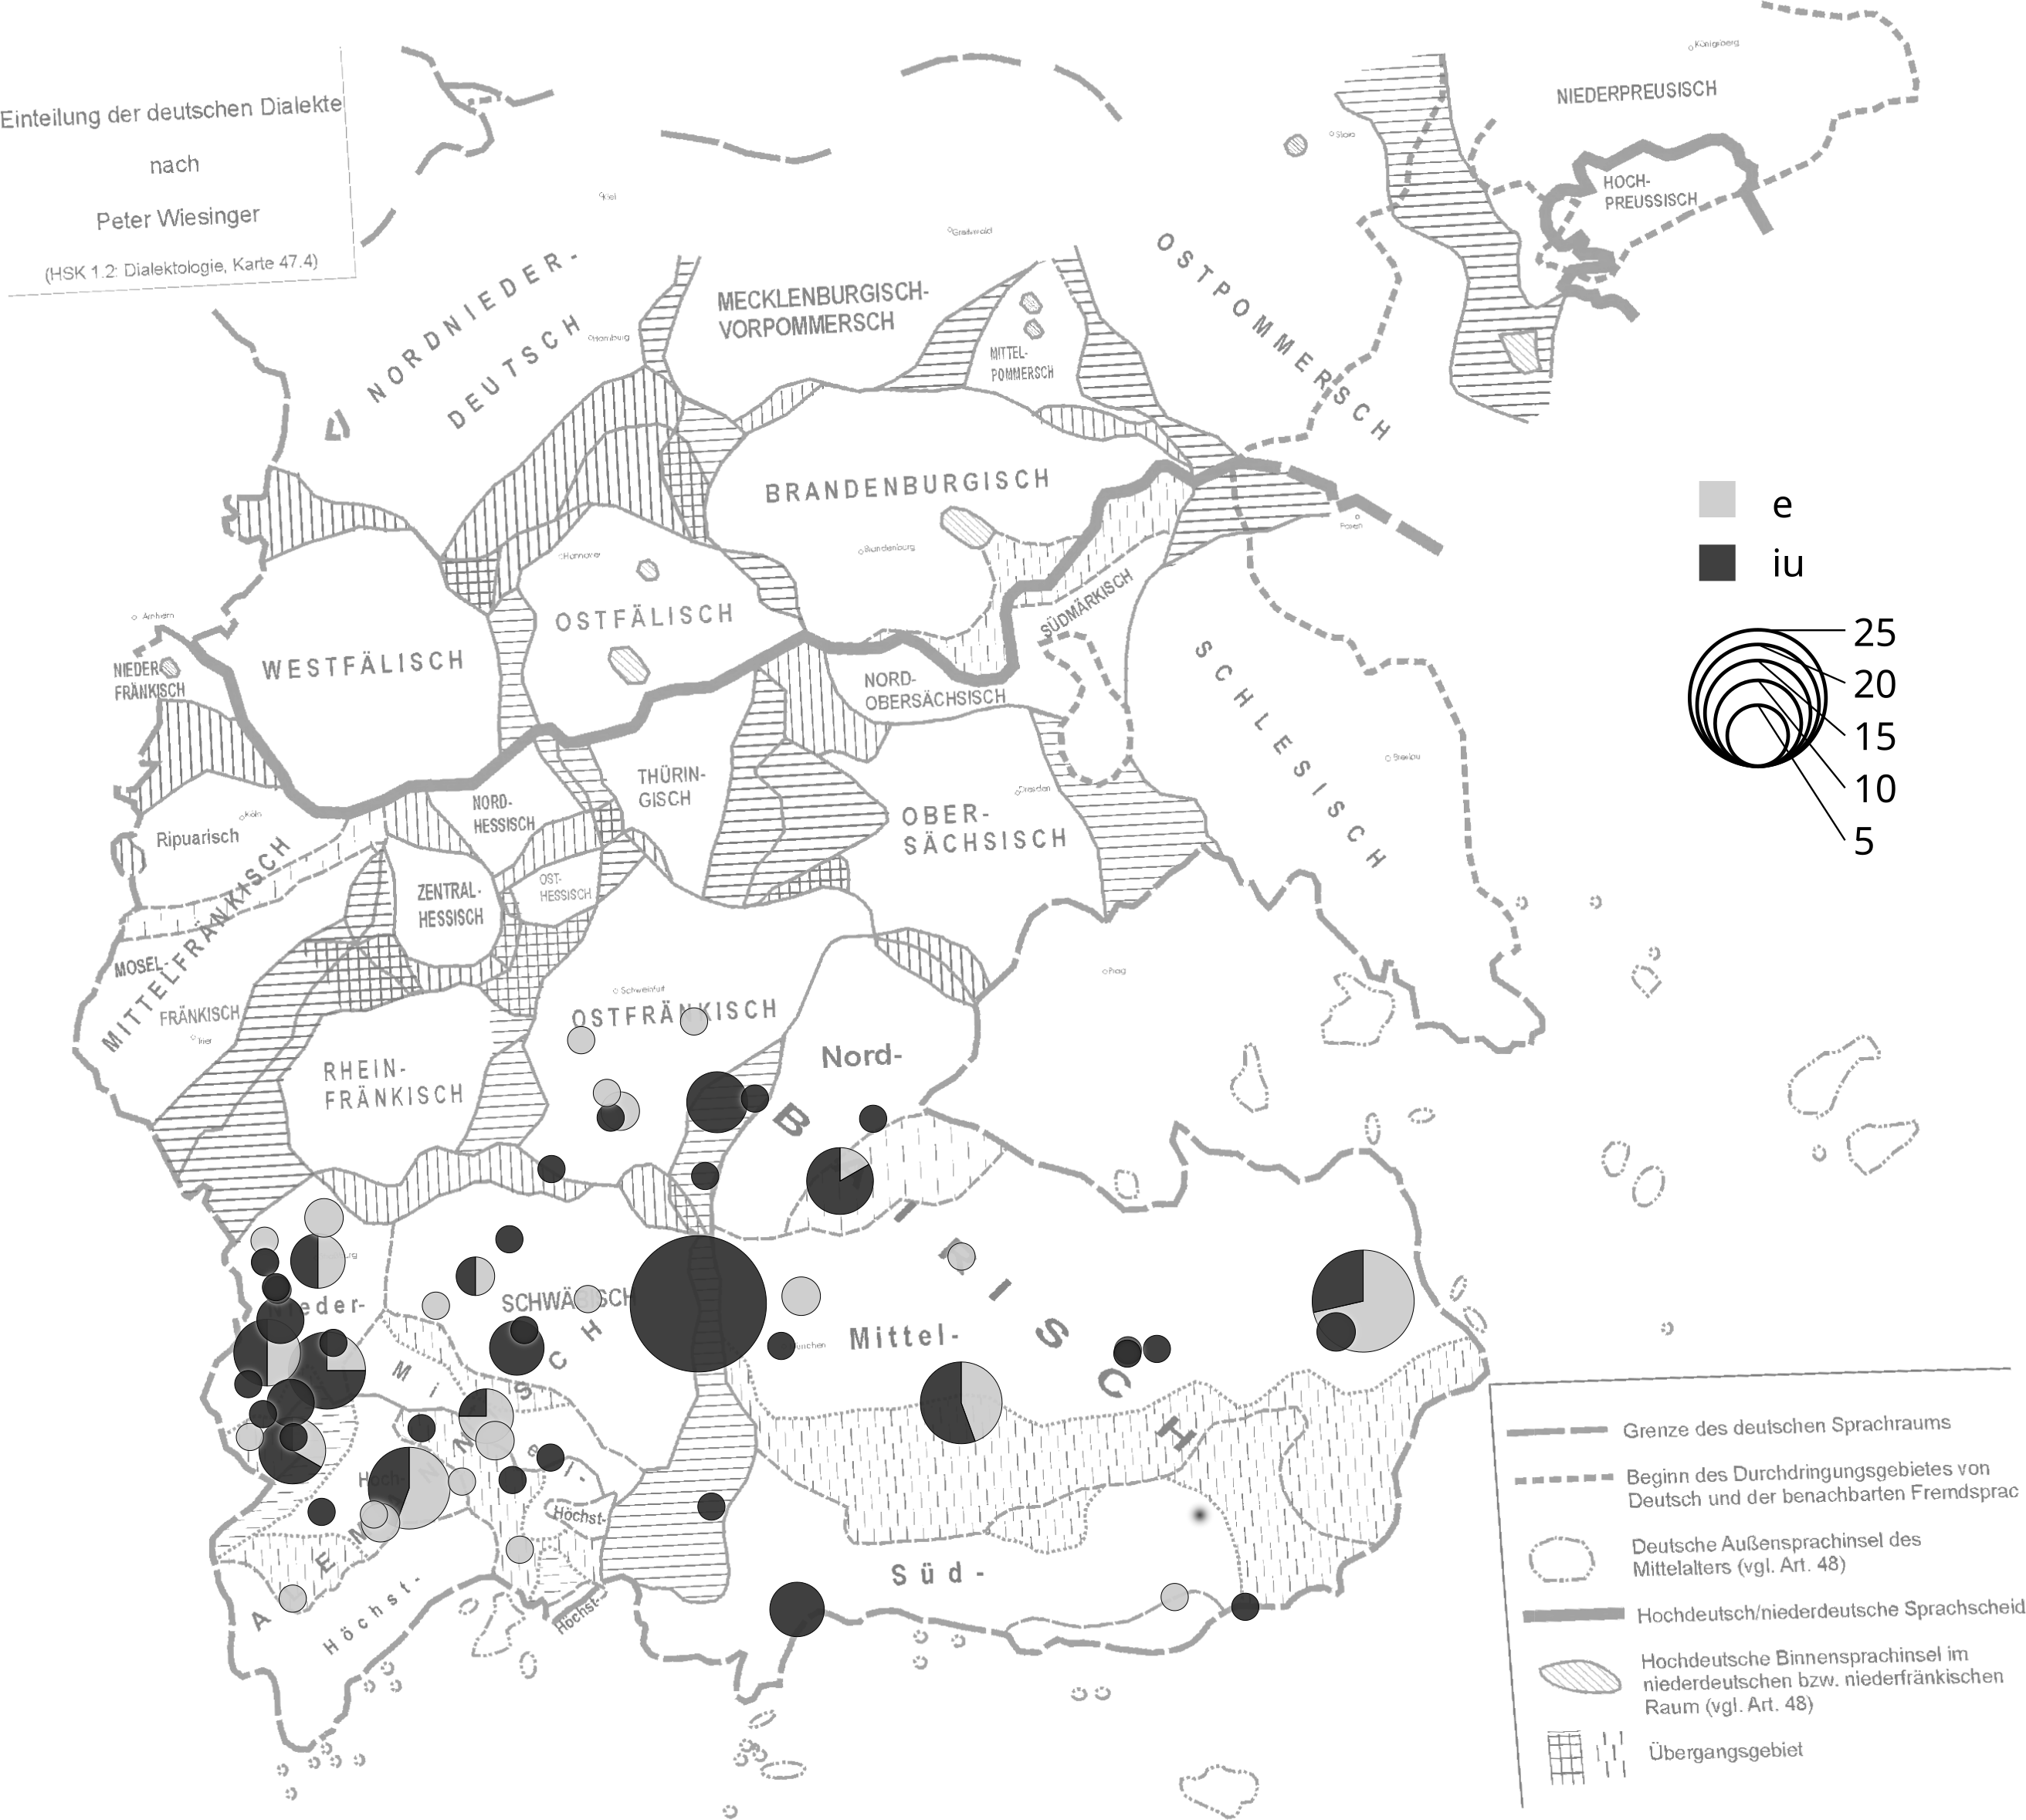
\includegraphics[
		width=.5\linewidth,
	]{./figures/2021-07-12_cao_beide_iu-quant.png}
}
\subfloat[\norm{bėide} als Konjunktion (\norm{bėide} \textsc{x} \norm{unde} \textsc{y})]{
	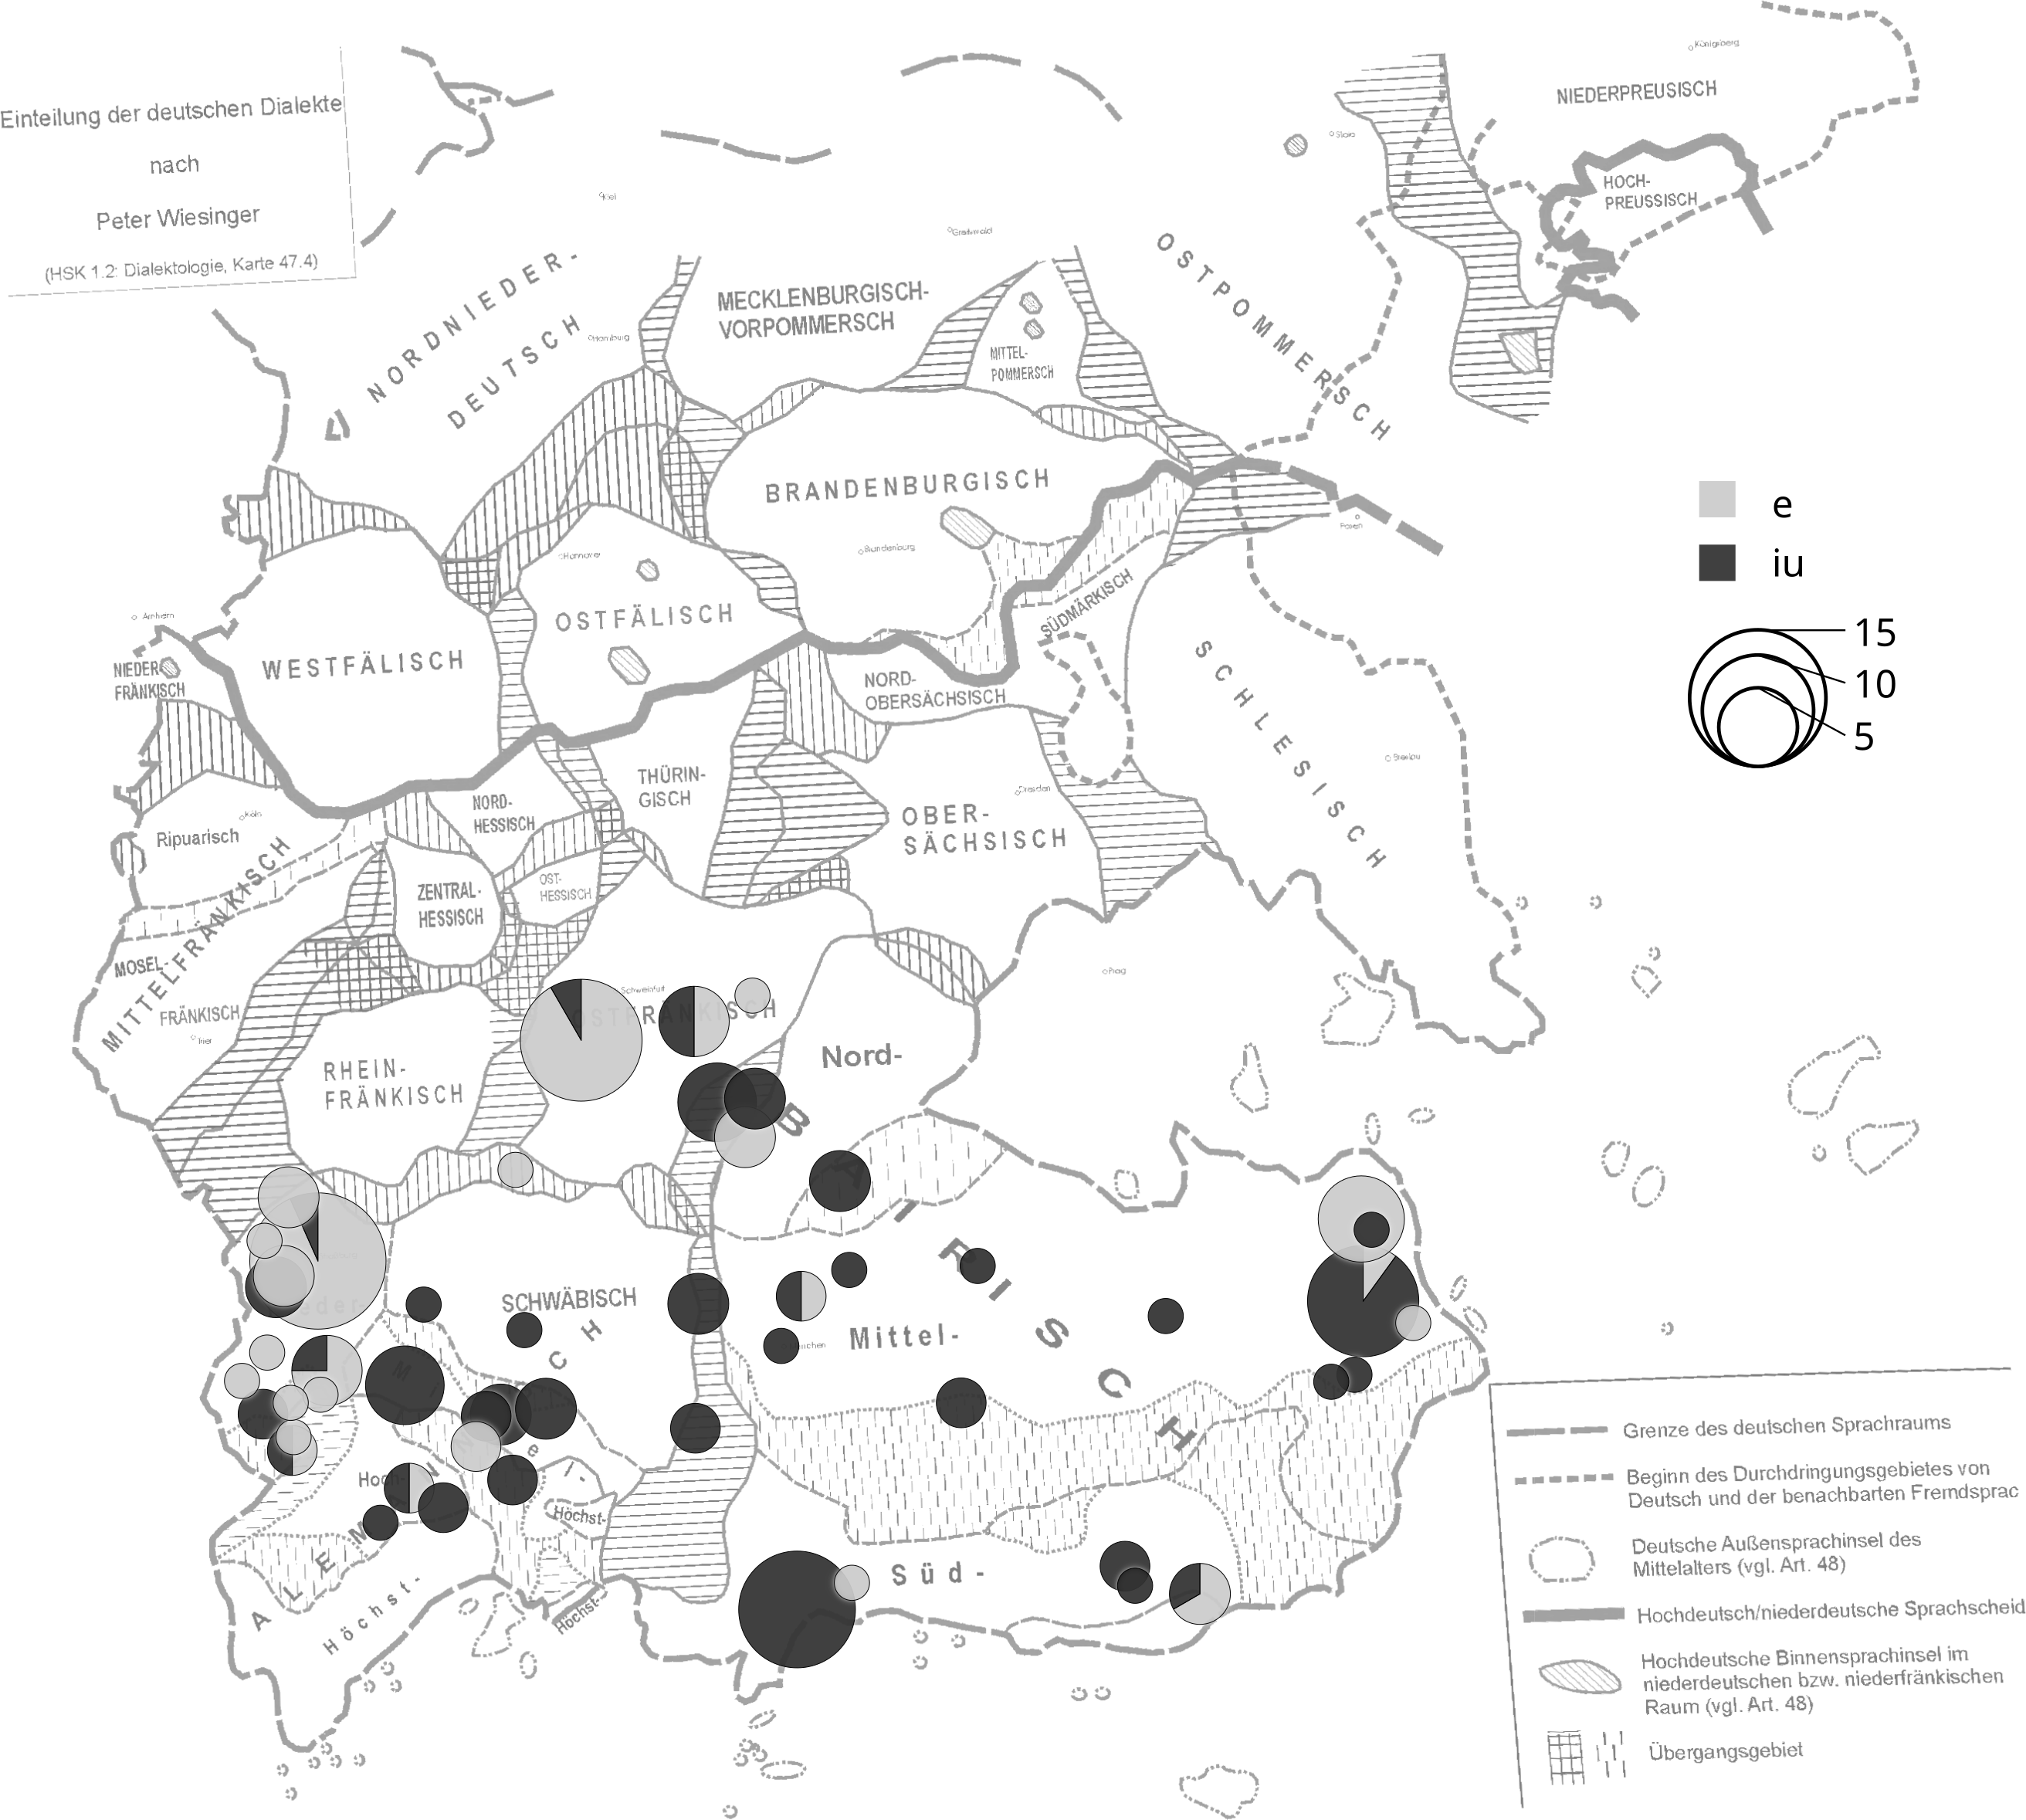
\includegraphics[
		width=.5\linewidth,
	]{./figures/2021-07-12_cao_beide_iu-conj.png}
}
\caption{Die geografische Verteilung von \norm{e}- und \norm{iu}-Flexionstypen}
\label{fig:cao_beide_geofunctypes}
\end{figure}
\end{landscape}
}

Darüber hinaus liegt in je einem Fall Variation zwischen einer Urkunde und
ihrer Kopie bei ansonsten gleichem Wortlaut \cref{ex:intraurkvar1} sowie
Variation innerhalb derselben Urkunde vor \cref{ex:intraurkvar2}. Beide
Urkunden stammen aus dem ostfränkischen Sprachraum und illustrieren das dortige
Neben\-einander beider Formen.

\begin{exe}
\ex \label{ex:intraurkvar1}
	\begin{xlist}
	\ex \label{ex:intraurkvar1_1}
		\let\eachwordthree\eachwordtwo
		\let\eachwordtwo\eachwordone
		\glll vnd daz wir deſte baz beide der ſtat zu Wirceburg vnd
				deme lande den Vride gevurdern mugen \\
			Vnd daz wir deſte baz beidu der ſtat zu Wirceburg/ Vnd
				dem lande den fride gevurdern mugen \\
			und dass wir desto besser beide der Stadt zu Würzburg und dem Land 
				den Frieden fördern können \\
		\trans `damit wir den Frieden sowohl in der Stadt Würzburg als
			auch im Land umso besser fördern können'
			\parencites(Nrn.~1126~AB, Würzburg, 1289)[414,36--38 bzw.~37--39]{cao2}
	\end{xlist}

\ex \label{ex:intraurkvar2}
	\begin{xlist}
	\ex \label{ex:intraurkvar2_1}
		\gll aller anſprache / immerewiclichen gelazen beidiv Ledic
				vnde vri \\
			aller Anklage {} immer.ewiglich gelassen beide ledig und frei \\
		\trans `für immer und ewig aller Anklage sowohl ledig als auch frei
			gelassen'
			\parencites(Nr.~2293, Bamberg, 1295)[420,23]{cao3}

	\ex \label{ex:intraurkvar2_2}
		\gll vnſer zinsgelt beide klein vnde groz \\
			unser Zinsgeld beide klein und groß \\
		\trans `unser Zinsgeld, sowohl kleines als auch großes'
			\parencites(Nr.~2293, Bamberg, 1295)[420.30]{cao3}
	\end{xlist}
\end{exe}

\subsection{Mit zwei Controllern}
\label{subsec:caokonj2ctrl}

Mit 59 Belegen ist die Koordination von zwei nominalen Elementen der häufigste
Anwendungsfall der Konstruktion \norm{bėide \dots\ unde} `sowohl \dots\
als auch' im untersuchten Material. Ein Beispiel für die hier diskutierten
Verwendungsweisen wird in \cref{ex:caokonj2ctrl} gegeben. Als Elemente, die
koordiniert werden, dienen einzelne Substantive \cref{ex:caokonj2ctrl_1},
Pronomina und Namen \cref{ex:caokonj2ctrl_2}, komplexe Nominalphasen
\cref{ex:caokonj2ctrl_3} oder auch freie Relativsätze \cref{ex:caokonj2ctrl_4}.
Gemeinsam ist den hier untersuchten Konjunkten, dass sie Controller enthalten.

\begin{exe}
\ex \label{ex:caokonj2ctrl}
	\begin{xlist}
	\ex \label{ex:caokonj2ctrl_1}
		\gll beidv̍ reben vn̄ garten \\
			beide Reben und Garten \\
		\trans `sowohl Reben als auch Garten'
			\parencites(Nr.~2353, Basel, 1296)[462,28--29]{cao3}

	\ex \label{ex:caokonj2ctrl_2}
		\gll beidiv ich / Vnd hainrich von meringen \\
			beide ich {} und Heinrich von Meringen \\
		\trans `sowohl ich als auch Heinrich von Meringen'
			\parencites(Nr.~1347, Kl.~Steingaden, Kr.~Weilheim-Schongau, 1291)[578,25]{cao1}

	\ex \label{ex:caokonj2ctrl_3}
		\gll beidv er / vn̄ oͮch alle die / den er ſvͥ gît \\
			beide er {} und auch alle die {} denen er sie gibt \\
		\trans `sowohl er als auch alle die, denen er sie gibt'
			\parencites(Nr.~1566, Hüfingen, Schwarzwald-Baar-Kr., 1292)[717,18]{cao2}

	\ex \label{ex:caokonj2ctrl_4}
		\gll bediv di nv lebent · vn̄ hernahe chvmftige ſint \\
			beide die nun leben {} und hernach künftig sind \\
		\trans `sowohl die nun leben als auch hernach künftig sind'
			\parencites(Nr.~1352, Wien, 1291)[580,8]{cao2}
	\end{xlist}
\end{exe}

\cref{tab:caokoordnomctrl} listet die Belegzahlen für \norm{bėide} und
\norm{bėidiu} in Abhängigkeit der Personenmerkmale der Konjunkte auf. Es ist
zwar mit \citet[626]{ksw2} davon auszugehen, dass die koordinierten Elemente
ursprünglich appositiv zu einem pronominal gebrauchten `beide' waren
(\norm{bėide}, \textsc{x} \norm{unde} \textsc{y}). Aus der Belegverteilung im
Urkundenmaterial ist jedoch nicht \fw{per se} zu schließen, dass konjunktional
gebrauchtes \norm{bėide} bei der Koordination von nominalen Elementen noch
regelmäßig kongruiert.

\begin{table}[tp]
\centering
\caption{Form nach Personenmerkmalen nominaler Konjunkte}
\begin{tabular}{l l r r r}
\toprule
Konjunkt 1
	& Konjunkt 2
	& bėid(e)
	& bėidiu
	& Summe
	\\
\midrule

% Gleiches Geschlecht
\Fsg\subM         & \Fpl\subM         &    &  1 &  1 \\
\Fsg\subM         & \Tsg.\MascM       &  3 &  1 &  4 \\
\Tsg.\MascM       & \Tsg.\MascM       &  3 &  3 &  6 \\
\Tsg.\MascM       & \Tpl.\MascM       &    &  1 &  1 \\
\Tsg.\FemF        & \Tsg.\FemF        &    &  1 &  1 \\
%                                        6    7   13

\midrule

% Unterschiedliches Geschlecht
\Fsg\subM         & \Tsg.\FemF        &    &  1 &  1 \\
\Fsg\subF         & \Tsg.\MascM       &  1 &    &  1 \\
\Tsg.\MascM       & \Tsg.\FemF        &    &  1 &  1 \\
\Tpl.\FemF        & \Tpl.\MascM       &    &  2 &  2 \\
%                                        1    4    5

\midrule

% Mit gleichem Genus und egalem Geschlecht
\Fsg\subM         & \Tpl.\MascA       &  3 &    &  3 \\
\Tsg.\MascA       & \Tsg.\MascA       &  1 &  1 &  2 \\
\Tsg.\MascA       & \Tpl.\MascA       &    &  1 &  1 \\
\Tsg.\MascM       & \Tpl.\MascA       &    &  1 &  1 \\
\Tpl.\MascA       & \Tpl.\MascA       &  9 &  5 & 14 \\
\Tpl.\MascM       & \Tpl.\MascA       &  1 &    &  1 \\
\Tsg.\MascM       & \Tpl.\NeutA       &  1 &    &  1 \\
%                                       15    8   23

\midrule

% Mit unterschiedlichem Genus und egalem Geschlecht oder unbelebt
\Tsg.\NeutA       & \Tpl.\MascA       &    &  1 &  1 \\
\Tsg.\MascM       & \Tsg.\NeutI       &    &  1 &  1 \\
\Tpl.\MascA       & \Tpl.\NeutI       &  1 &  5 &  6 \\
%                                        1    7    8

\midrule

% Gleiches Genus (unbelebt)
\Tsg.\FemI        & \Tsg.\FemI        &    &  1 &  1 \\
\Tsg.\NeutI       & \Tsg.\NeutI       &  1 &    &  1 \\
\Tsg.\MascI       & \Tpl.\MascI       &  1 &    &  1 \\
%                                        2    1    3

\midrule

% Unterschiedliches Genus (unbelebt)
\Tsg.\MascI       & \Tsg.\NeutI       &    &  1 &  1 \\
\Tsg.\FemI        & \Tsg.\NeutI       &  1 &  1 &  2 \\
\Tsg.\NeutI       & \Tsg.\FemI        &    &  3 &  3 \\
\Tpl.\MascI       & \Tpl.\FemI        &  2 &    &  2 \\
\Tpl.\MascI       & \Tsg.\NeutI       &  1 &    &  1 \\
\Tpl.\FemI        & \Tsg.\MascI       &    &  1 &  1 \\
\Tpl.\FemI        & \Tpl.\MascI       &    &  1 &  1 \\
%                                        4    7   11

\midrule
\mc{2}{l}{Summe}                      & 29 & 34 & 63 \\
\bottomrule
\end{tabular}
\label{tab:caokoordnomctrl}
\end{table}

Der erste Abschnitt in \cref{tab:caokoordnomctrl} enthält Konjunkte mit
gleichwertigen Genus- und Sexus\-merkmalen ($\MascM+\MascM{}$ und
$\FemF+\FemF$). Anders als bisher beobachtet, steht in 54\,\% der Fälle die
ansonsten neutrale Form \norm{bėidiu}. Im dritten Abschnitt, der mindestens ein
Element mit irrlevantem Sexus enthält, das formal jedoch maskulin ist (\MascA,
zum Beispiel
% \norm{liute}
\norm{lǖte} `Leute',
% \norm{burgære}
\norm{burgǟre} `Bürger'), und einem weiteren solchen oder einem
maskulin-männlichen Element ($\MascA+\MascA{}$ und $\MascM+\MascA$)
häufen sich dagegen die Belege bei \norm{bėid(e)}, das 65\,\% der für diesen
Kontext belegten Formen ausmacht. Im letzten Abschnitt der Tabelle, der
unbelebte Elemente mit unterschiedlichem Genus enthält, wird anders als zuvor
\norm{bėidiu} nicht klar favorisiert: Mit 58\,\% für \norm{bėidiu} sind die
Verhältnisse nahezu ausgeglichen. Insgesamt ergibt sich keine klare, von
Personenmerkmalen abhängige Verteilung.

Für den zweiten Abschnitt mit unterschiedlichen Geschlechtsmerkmalen belebter
Konjunkte scheint eine klare Präferenz für \norm{bėidiu} vorzuliegen, die
ähnlich eindeutig zu sein scheint wie bei der Verwendung von \norm{bėide} als
Quantor. Dasselbe gilt für die vierte Gruppe mit Kombinationen mit
unspezifischem Geschlecht sowie belebten mit unbelebten Konjunkten enthalten.
Sollte dies als Evidenz für Gender Resolution dienen? \citet[187]{gjelsten1980}
räumt in ihrer Kritik an \posscite{askedal1974} Arbeit zu konjunktionalem
\norm{bėide} ein, dass bei substantivischen Konjunkten nicht klar zwischen
pronominalem Gebrauch (\norm{bėide}, \textsc{x} \norm{unde}~\textsc{y}) und
konjunktionalem (\norm{bėide}~\textsc{x} \norm{unde}~\textsc{y}) unterschieden
werden kann. Angesichts der recht homogenen Verteilung der Formen \norm{bėide}
und \norm{bėidiu} ist aber nicht davon auszugehen, dass ausgerechnet hier
plötzlich regelmäßig Kongruenz zwischen \norm{bėide} und den Konjunkten
herrscht.

\cref{tab:caokoordnomctrl} trennt nicht nach Kasus; die folgende
\cref{tab:caokoordnomctrlcase} stellt die Verteilung zumindest der
Kombinationen von Konjunkten dar, die eine klare Zuordnung des Geschlechts
erlaubt. Belege mit Gruppenbezeichnungen wie \norm{lǖte} `Leute
(\MascA)', \norm{arme} `Arme (\MascA)' und \norm{alle die, den ęr si
gibet} `alle die (\MascA?), denen er sie gibt' sowie Kombinationen von
belebten und unbelebten Konjunkten wie in \norm{lǖte unde guet} `Leute
(\MascA) und Gut (\NeutI)' wurden nicht gewertet. Bei allen diesen Belegen ist
ohnehin nur \norm{bėide} für den Nom., Akk.\ und den Dat.\ belegt; für den
Gen.\ liegen keine Belege vor.

\begin{table}
\centering
\caption{Form nach dem Kasus nominaler Konjunkte}
\begin{tabularx}{\linewidth}{
	l
	R R c R R
	c
	R R c R R
	r
}
\toprule
\mr{3}{*}[-1ex]{}
	& \mc{5}{c}{belebt}
	& % --
	& \mc{5}{c}{unbelebt}
	& \mr{3}{*}[-1ex]{Summe}
	\\

\cmidrule{2-6}
\cmidrule{8-12}

%
	& \mc{2}{c}{gleich}
	& % --
	& \mc{2}{c}{verschieden}
	& % --
	& \mc{2}{c}{gleich}
	& % --
	& \mc{2}{c}{verschieden}
	& % --
	\\

\cmidrule{2-3}
\cmidrule{5-6}
\cmidrule{8-9}
\cmidrule{11-12}

%
	& bėid(e)
	& bėidiu
	& % --
	& bėid(e)
	& bėidiu
	& % --
	& bėid(e)
	& bėidiu
	& % --
	& bėid(e)
	& bėidiu
	& % --
	\\

\midrule

\Nom
	& 4
	& 4
	& % --
	& 1
	& 2
	& % --
	& %
	& %
	& % --
	& %
	& 3
	& 14
	\\

\midrule

\Acc
	& 2
	& %
	& % --
	& %
	& %
	& % --
	& 3
	& %
	& % --
	& 2
	& 3
	& 10
	\\

\midrule

\Dat
	& %
	& 2
	& % --
	& %
	& 1
	& % --
	& %
	& %
	& % --
	& 1
	& 1
	& 5
	\\

\midrule

\Gen
	& %
	& 1
	& % --
	& %
	& 1
	& % --
	& %
	& %
	& % --
	& 1
	& %
	& 3
	\\

\midrule

Summe
	& 6
	& 7
	& % --
	& 1
	& 4
	& % --
	& 3
	& %
	& % --
	& 4
	& 7
	& 32
	\\

\bottomrule
\end{tabularx}
\label{tab:caokoordnomctrlcase}
\end{table}

Bei der Betrachtung nach Kasus ergibt sich für den Nom./Akk.\ keine klare
Präferenz bei belebten Konjunkten mit gleichem Geschlecht, da hier die
Verhältnisse nahezu ausgeglichen sind. Für Kombinationen mit verschiedenem
belebten Geschlecht liegen zu wenige Belege vor, um eine Regel aufzustellen.
Dasselbe gilt für die drei Belege für \norm{bėide} bei gleichem unbelebten
Genus. Bei verschiedenem unbelebten Genus entfällt der Großteil der Belege auf
\norm{bėidiu}.

Darüber hinaus liegen allerdings auch Belege für \norm{bėide} und \norm{bėidiu}
im Dativ und Genitiv vor. Wenn \norm{bėide} entsprechend der formalen
Merkmale der jeweiligen NP flektieren würde, dürften diese Formen nicht
auftreten. Nun ist nicht auszuschließen, dass die Flexionskategorie Kasus in
diesem Fall wegfällt, das Geschlecht beziehungsweise Genus der Konjunkte aber
trotzdem eine Auswirkung auf die Form der Konjunktion hat. Abgesehen von je
einem Beleg für \norm{bėide} bei verschiedenem unbelebten Genus steht in den
vereinzelten belegten Fällen \norm{bėidiu}.

Insgesamt ist keine deutliche Häufung auf \norm{bėide} bei gleichem belebtem
Geschlecht sowie auf \norm{bėidiu} bei unbelebtem Bezug unabhängig vom Genus
auszumachen, wie dies bei der quantifizierenden Verwendung der Fall war.
Angesichts der vereinzelten Belege in den einzelnen Kasusfeldern kann wohl auch
für belebte Konjunkte mit verschiedenem Geschlecht keine Regel für das
Auftreten von \norm{bėidiu} abgeleitet werden. Wenn sich Belege mit
pronominalem \norm{bėide} eingeschlichen haben sollten, treten diese nicht klar
aus der Statistik hervor.

\subsection{Mit zwei Targets}
\label{subsec:caobeidkoordtarg}

Parallel zur Auswertung in \cref{subsubsec:beid2p2coordncao} zum Einfluss der
Personenmerkmale auf die Form von \norm{bėide} beim indirekten Bezug auf
kombinierte nominale Controller lassen sich auch für die Konjunktion
\norm{bėide} solche Konjunkte untersuchen, die selbst keine Personenmerkmale
definieren, sondern Kongruenz\-targets darstellen. In der Stichprobe sind dies
konkret verschiedene Arten von Adjektiven, die in \cref{ex:caobeidkoordtarg}
beispielhaft angeführt sind: vorangestellt attributive
\cref{ex:caobeidkoordtarg_1}, nachgestellt attributive
\cref{ex:caobeidkoordtarg_2} und prädikative \cref{ex:caobeidkoordtarg_3},
wobei die Zuordung bei Nachstellung nicht immer eindeutig ist.

\begin{exe}
\ex \label{ex:caobeidkoordtarg}
	\begin{xlist}
	\ex \label{ex:caobeidkoordtarg_1}
		\gll beide geiſtliches / vn̄ wertliches gerihtes \\
			beide geistlich-\Gen.\Sg.\NeutI.\St{} {} und
			weltlich-\Gen.\Sg.\NeutI.\St{} Gericht-\Gen.\Sg{}[\NeutI] \\
		\trans `sowohl geistlichen als auch weltlichen Gerichts'
			\parencites(Nr.~1764, Bamberg, 1293)[71,26]{cao3}

	\ex \label{ex:caobeidkoordtarg_2}
		\gll erberge leut peideu gaiſtlich vnd wertlich \\
			ehrenhafte Leute[\Nom.\Pl.\MascA] beide geistlich[\Nom.\Pl.\MascA]
			und weltlich[\Nom.\Pl.\MascA] \\
		\trans `sowohl geistliche und weltliche ehrenhafte Leute'
			\parencites(Nr.~1153, Engelthal, Kr.~Nürnberger Land, 1289)[431,44]{cao2}

	\ex \label{ex:caobeidkoordtarg_3}
		\gll vnde hat {div ſelben} gvͦt \textelp{} aller anſprache /
			immerewiclichen gelazen beidiv Ledic vnde vri \\
			und hat dieselben Gut[\Acc.\Pl.\NeutI] {} aller Anklage {}
			immer.und.ewig gelassen beide ledig[\Acc.\Pl.\NeutI] und
			frei[\Acc.\Pl.\NeutI] \\
		\trans `und hat dieselben Güter \textelp{} immer und ewig sowohl
			ledig als auch frei von aller Anklage gelassen'
			\parencites(Nr.~2293, Bamberg, 1295)[420,21--23]{cao3}
	\end{xlist}
\end{exe}

Auch für die Koordination von Adjektiven lässt sich keine regelmäßige
Korrespondenz zwischen der Kombination bestimmter Personenmerkmale und
konjunktional gebrauchtem \norm{bėide} feststellen, wie
\cref{tab:caokoordtarg} zeigt. Für Konjunkte mit gleichen Genus- und
Sexusmerkmalen liegt nur ein einziger Beleg vor; bei der Konjunktion von
maskulinen Targets mit beliebigem Sexus sind die Verhältnisse nahezu
ausgeglichen, insofern in 57\,\% der Fälle \norm{bėide} belegt ist. Bei den
unbelebten Targets mit unterschiedlichem Genus steht in 64\,\% der Belege
\norm{bėidiu}.

\begin{table}
\centering
\caption{Form nach Personenmerkmalen adjektivischer Konjunkte}
\begin{tabular}{l l r r r}
\toprule
Konjunkt 1
	& Konjunkt 2
	& bėid(e)
	& bėidiu
	& Summe
	\\
\midrule

% Gleiches Geschlecht
\FemF.\Sg        & \FemF.\Sg  &  1 &    &  1 \\

\midrule

% Mit gleichem Genus und egalem Geschlecht
\MascA.\Pl       & \MascA.\Pl &  4 &  3 &  7 \\

\midrule

% Gleiches Genus (unbelebt)
\MascI.\Sg       & \MascI.\Sg &  1 &  3 &  4 \\
\FemI.\Sg        & \FemI.\Sg  &    &  1 &  1 \\
\NeutI.\Sg       & \NeutI.\Sg &  4 &  1 &  5 \\
\NeutI.\Pl       & \NeutI.\Pl &    &  1 &  1 \\
%                                5    6   11

\midrule
\mc{2}{l}{Summe}              & 10 &  9 & 19 \\
\bottomrule
\end{tabular}
\label{tab:caokoordtarg}
\end{table}

% Blickt man auch hier auf die Verteilung der Belege nach Kasus, ergibt sich,
% dass von einer klaren Präferenz für \norm{bėidiu} bei unbelebtem Bezug wie
% bei der Verwendung als Quantor keine Rede sein kann. Auch in
% \cref{tab:caokoordtargcase} wurden Gruppenbezeichnungen wie \norm{lǖte}
% `Leute (\MascA)' ignoriert. Neben einem einzelnen \norm{bėide}-Beleg für
% die Kombination von zwei Konjunkten mit gleichem Geschlecht im Nominativ
% liegen lediglich Belege für gleiches unbelebtes Genus vor. Diese verteilen
% sich insgesamt gleichmäßig auf \norm{bėide} und \norm{bėidiu}, wobei
% zumindest im Akk.\ drei von vier Belegen auf \norm{bėidiu} entfallen.
% Umgekehrt liegen im Gen.\ drei von vier Belegen für \norm{bėide} vor, im
% Dat.\ zwei von drei für \norm{bėidiu}. Bei den hier nicht aufgeführten
% Belegen mit unbestimmtem Geschlecht entfallen im Nom.\ zwei auf \norm{bėide},
% drei auf \norm{bėidiu} und im Dat.\ zwei auf \norm{bėide}. Für den Akk.\ und
% den Gen.\ liegen keine Belege vor.

% \begin{table}
% \centering
% \caption{Verteilung der `beide'-Formen in Abhängigkeit des Kasus
% adjektivischer Konjunkte}
% \begin{tabularx}{.75\linewidth}{
% 	l
% 	R R % c R R
% 	c
% 	R R % c R R
% 	r
% }
% \toprule
% \mr{3}{*}[-.5ex]{}
% 	& \mc{2}{c}{belebt} % \mc{5}{c}{belebt}
% 	& % --
% 	& \mc{2}{c}{unbelebt} % \mc{5}{c}{unbelebt}
% 	& \mr{3}{*}[-.5ex]{Summe}
% 	\\

% % \cmidrule{2-3} % \cmidrule{2-6}
% % \cmidrule{5-6} % \cmidrule{8-12}

% % %
% % 	& \mc{2}{c}{gleich}
% % 	% & % --
% % 	% & \mc{2}{c}{verschieden}
% % 	& % --
% % 	& \mc{2}{c}{gleich}
% % 	% & % --
% % 	% & \mc{2}{c}{verschieden}
% % 	& % --
% % 	\\

% \cmidrule{2-3}
% \cmidrule{5-6}
% % \cmidrule{8-9}
% % \cmidrule{11-12}

% %
% 	& bėid(e)
% 	& bėidiu
% 	% & % --
% 	% & bėid(e)
% 	% & bėidiu
% 	& % --
% 	& bėid(e)
% 	& bėidiu
% 	% & % --
% 	% & bėid(e)
% 	% & bėidiu
% 	& % --
% 	\\

% \midrule

% \Nom
% 	& 1
% 	& %
% 	% & % --
% 	% & %
% 	% & %
% 	& % --
% 	& 1
% 	& %
% 	% & % --
% 	% & %
% 	% & %
% 	& 2
% 	\\

% \midrule

% \Acc
% 	& %
% 	& %
% 	& % --
% 	% & %
% 	% & %
% 	% & % --
% 	& 1
% 	& 3
% 	% & % --
% 	% & %
% 	% & %
% 	& 4
% 	\\

% \midrule

% \Dat
% 	& %
% 	& %
% 	% & % --
% 	% & %
% 	% & %
% 	& % --
% 	& 1
% 	& 2
% 	% & % --
% 	% & %
% 	% & %
% 	& 3
% 	\\

% \midrule

% \Gen
% 	& %
% 	& %
% 	% & % --
% 	% & %
% 	% & %
% 	& % --
% 	& 3
% 	& 1
% 	% & % --
% 	% & %
% 	% & %
% 	& 4
% 	\\

% \midrule

% Summe
% 	& 1
% 	& %
% 	% & % --
% 	% & %
% 	% & %
% 	& % --
% 	& 6
% 	& 6
% 	% & % --
% 	% & %
% 	% & %
% 	& 13
% 	\\

% \bottomrule
% \end{tabularx}
% \label{tab:caokoordtargcase}
% \end{table}

\subsection{Rein syntaktischer Kontext}
\label{subsec:caobeidquantsyncont}

Im Urkundenmaterial kommt neben der Konjunktion von Controllern und Targets,
die Personenmerkmale definieren beziehungsweise widerspiegeln, auch die
Konjunktion solcher Elemente vor, die keinerlei Personenmerkmale definieren.
Die Konstruktion \norm{bėide \dots\ unde} `sowohl \dots\ als auch' hat
hier insofern funktionalen Charakter, als \norm{bėide} als Fokuspartikel dient,
die die Zweiheit der Optionen betont \autocites(siehe auch
\cref{sec:ovwbeideconj})[425--428]{johannessen2005}.
% 
% \begin{exe}
% \ex \label{ex:beidenoagr}
% 	\begin{xlist}
% 	\ex[]{(allen) beiden$_{i+j}$, Sabine$_i$ und Peter$_j$}
% 		\label{ex:beidenoagr_1}
% 
% 	\ex[*]{(allen) beiden$_{i+j}$, hier$_i$ und in Berlin$_j$}
% 		\label{ex:beidenoagr_2}
% 	\end{xlist}
% \end{exe}
% 
Im exzerpierten Material kommt \norm{bėide} in diesem Zusammenhang mit
Temporaladverbien \cref{ex:caokoordsyn_1}, Lokaladverbien
\cref{ex:caokoordsyn_2} und Präpositionalphrasen
\crefrange{ex:caokoordsyn_2}{ex:caokoordsyn_3} vor.

\begin{exe}
\ex \label{ex:caokoordsyn}
	\begin{xlist}
	\ex \label{ex:caokoordsyn_1}
		\gll beide vor vn̄ noͤch \\
			beide vor und nach \\
		\trans `sowohl davor als auch danach'
			\parencites(Nr.~N~689, Straßburg, 1295)[499,25]{cao5}

	\ex \label{ex:caokoordsyn_2}
		\gll beide da vn̄ an allin ſteitin \\
			beide da und an allen Stätten \\
		\trans `sowohl dort als auch an allen \textins{anderen} Orten'
			\parencites(Nr.~N~321, Rosheim, Dépt.~Bas-Rhin, 1286)[245,24]{cao5}

	\ex \label{ex:caokoordsyn_3}
		\gll baidev zv Dorfe vnd ze velde \\
			beide zu Dorf-\Dat.\Sg{} und zu Feld-\Dat.\Sg{} \\
		\trans `sowohl im Dorf als auch auf dem Feld'
			\parencites(Nr.~3319, Michelstetten, Bz.~Mistelbach, 1299)[461,28]{cao4}
	\end{xlist}
\end{exe}

In \cref{tab:caokoordsyn} werden der Vollständigkeit halber die Belegzahlen pro
Kombination der Wortart oder des Phrasentyps der Konjunkte aufgelistet. Eine
auffällige Häufung, die Anlass dazu geben würde, eine Präferenz in Abhängigkeit
der Konjunkte anzunehmen, ist auch hier nicht gegeben. Mit Ausnahme von zwei
bairisch-österreichischen Belegen aus Fallbach (Bz.~Mistelbach) und eines aus
St.~Paul im Lavanttal (Bz.~Wolfsberg) stammen die Belege für die Form
\norm{bėide} sämtlich aus dem alemannischen Sprachraum. Die Belege für
\norm{bėidiu} stammen umgekehrt hauptsächlich aus dem bairischen Sprachraum.

\begin{table}
\centering
\caption{Form nach Wortart adverbialer und präpositionaler Konjunkte}
\begin{tabular}{l l r r r}
\toprule
Konjunkt 1
	& Konjunkt 2
	& bėid(e)
	& bėidiu
	& Summe
	\\
\midrule

Adv     & Adv     &  2 &  1 &  3 \\

\midrule

PP      & AdvP    &  2 &    &  2 \\
AdvP    & PP      &  1 &    &  1 \\
%                    3    0    3

\midrule

PP      & PP      & 10 & 27 & 37 \\

\midrule
\mc{2}{l}{Summe}  & 15 & 28 & 43 \\
\bottomrule
\end{tabular}
\label{tab:caokoordsyn}
\end{table}

\subsection{Zusammenfassung}

Die aus dem \CAO{} exzerpierten Belege zu \norm{bėide} als Konjunktion
bestätigen die in \citet[626--627]{ksw2} formulierte Beobachtung, dass die Form
in diesem Kontext nicht mehr nach grammatischen Kriterien variiert, sondern
freie Variation zwischen \norm{bėide} und \norm{bėidiu} vorliegt. Weder mit
koordinierten Controllern noch mit koordinierten Targets wird eine eindeutige
Abhängigkeit der Form der Konjunktion von den Personenmerkmalen der Konjunkte
deutlich. Dass der Aspekt von \norm{bėide} als Fokuspartikel
\autocites(siehe auch \cref{sec:ovwbeideconj})[425--428]{johannessen2005} in
diesem Kontext vorherrscht, ist auch daran zu erkennen, dass \norm{bėide}
regelmäßig mit solchen Konjunkten auftritt, die keinerlei Personenmerkmale
definieren oder reflektieren, sodass kein Kontext vorliegt, in dem Kongruenz
angewendet werden kann.

Auch die geografische Verteilung betreffend decken sich die
\CAO{}-Belege mit den Aussagen in \citet[627--628]{ksw2}. Belege für
den Typ \norm{bėide} verteilen sich vor allem auf das
\mbox{(Nieder-)}\allowbreak{}Alemannische und Ostfränkische, im bairischen und
schwäbischen Sprachraum steht dagegen hauptsächlich \norm{bėidiu}. Ein
Unterschied zwischen \norm{-e} und \norm{-iu} anhand der syntaktischen Funktion
von \norm{bėide} macht sich nur insofern bemerkbar, als die Form bei
konjunktionalem Gebrauch in den Belegen zu Straßburg, Konstanz, Salzburg und
Wien deutlich erstarrt erscheint, während beim Quantor zumindest an den drei
zuletzt genannten Orten beide Flexionsformen auftreten.
